\documentclass[11pt, oneside]{article}   	% use "amsart" instead of "article" for AMSLaTeX format
\usepackage{hyperref}
\usepackage{geometry}                		% See geometry.pdf to learn the layout options. There are lots.
\geometry{letterpaper}                   		% ... or a4paper or a5paper or ... 
%\geometry{landscape}                		% Activate for rotated page geometry
%\usepackage[parfill]{parskip}    		% Activate to begin paragraphs with an empty line rather than an indent
\usepackage{graphicx}				% Use pdf, png, jpg, or eps§ with pdflatex; use eps in DVI mode
								% TeX will automatically convert eps --> pdf in pdflatex		
\usepackage{amssymb}

%SetFonts

%SetFonts


\title{$V-E+F=6757 - 13086 + 6331 = 2$}
\author{\today}
\date{}							% Activate to display a given date or no date

\begin{document}
\maketitle



\begin{figure}[htbp] %  figure placement: here, top, bottom, or page
   \centering
   \begin{minipage}[c]{0.8\textwidth}
{\scriptsize
\begin{verbatim}
[2681,2677,-4299,-2678]
[-2677,2679,-2682,4302]
[2678,2673,-4297,-2674,4298,-6532]
[-2673,2675,-2679,-4301,6535]
[2674,2670,-6530,-2671]
[-2670,2672,-2676,-12524]
[2671,2667,-6529,-2668]
[-2667,2669,-2672,9470]
[2668,2665,6529,-2666,6531,-4298,3933,-3932,4297,4299,-8943,5803,2741,-2740,5804,-2743, 
-12509,-3971,-10971,-10968,3970,3965,-10965,-3967,10967,3964,-10964,3959,-10806,-3960, 
-6032,6033,11280,-10960,5202,3950,10962,1847,12960,1844,-13048,-1846,-12949,-4992,12948, 
-4993,-7395,7394,3938,3934,11870,-3935,-12714,-7437,-9727,-9725,10566,-5141,5408,5139,
5406,5142,5404,5401,12212,-5403,12213,-11614,5400,5396,-11612,4398,-11609,-4399,11610,
10379,12940,10378,12942,10376,-1537,1536,-10377,1539,7184,-7183,-2362,-2358,-11590,2359,
-11591,5159,-11592,-5158,12765,-5156,12207,-4794,508,-507,-4790,-3322,4791,-3324,-5153,
-5150,5962,5152,-5960,-5964,-5149,5148,2321,2316,-9381,2314,9380,2312,9383,-2313,9385,
-5204,9387,9531,9946,-6247,-9945,6245,-10250,6248,10490,6250,-10491,-6733,10489,6734,
10486,2553, -10700,-2552,-10697,-9527,10698,9587,-11579,9585,-529,528,-9586,11545,
11578,5347,-12232, -5344,-11171,-5349,-8997,-8994,359,-358,-8992,-361,8993,-5350,-11520,
8064,11522,7742,-10485,-7743,-5542,-5540,3442,3439,-5537,-3441,5539,8056,-10959,8053,
10958,-8054,-9989,6976,9990,-6975,-1678,1679,-6978,-8824,-9101,-8826,9100,-8829,-9750,
9749,-11536,9753,8834,-8832,-9755,-8835,-8851,-8849,3678,-3677,-4716,-4713,43,-42,-1638,
-45,-1635,1637,-9686,4145,-9330,4143,-9326,4140,-9324,-4142,9325,-1535,11008,1534,
-11009,9428,5058,-5057,-6030,-5059,6031,-5061,10230,-5065,-9925,-8561,12422,8560,-12421,
-9920,10882,9922,-10881,-10884,12386,-10886,-6612,6611,10259,-10260,-4643,4641,8047,4644]
[42,-43,46]
[45,-44,-7324,-49]
[44,-46,48,-3676,3677]
[-48,47,-3679,50,-3682,54,4356]
	....  ....

[-56,55,4358,59,3684,2662,-2664,-2661]
[-55,57,-58,6615]
[58,-59,7325,7327,-11319,-5477,4518,4514,-5472,-4516,5474]
[358,-359,362]
\end{verbatim}}
\end{minipage}
   \caption{A portion of the computed list of 2-cells of Figure~\ref{fig:2Dcells}, each one described by an array of signed indices of edges. Each one correspond to a column of the signed buondary matrix $\partial_2$, with elements in $\{-1,0,1\}$. The matrix $\partial_2$ is $13086 \times 6331$, and contains $82,\!847,\!466$ elements, including $26,\!172$ non-zeros, with a filling ratio equal to $0.03159\%$. The size of the representation is exactly $2E$.}
   \label{fig:example}
\end{figure}

\begin{figure}[htbp] %  figure placement: here, top, bottom, or page
   \centering
   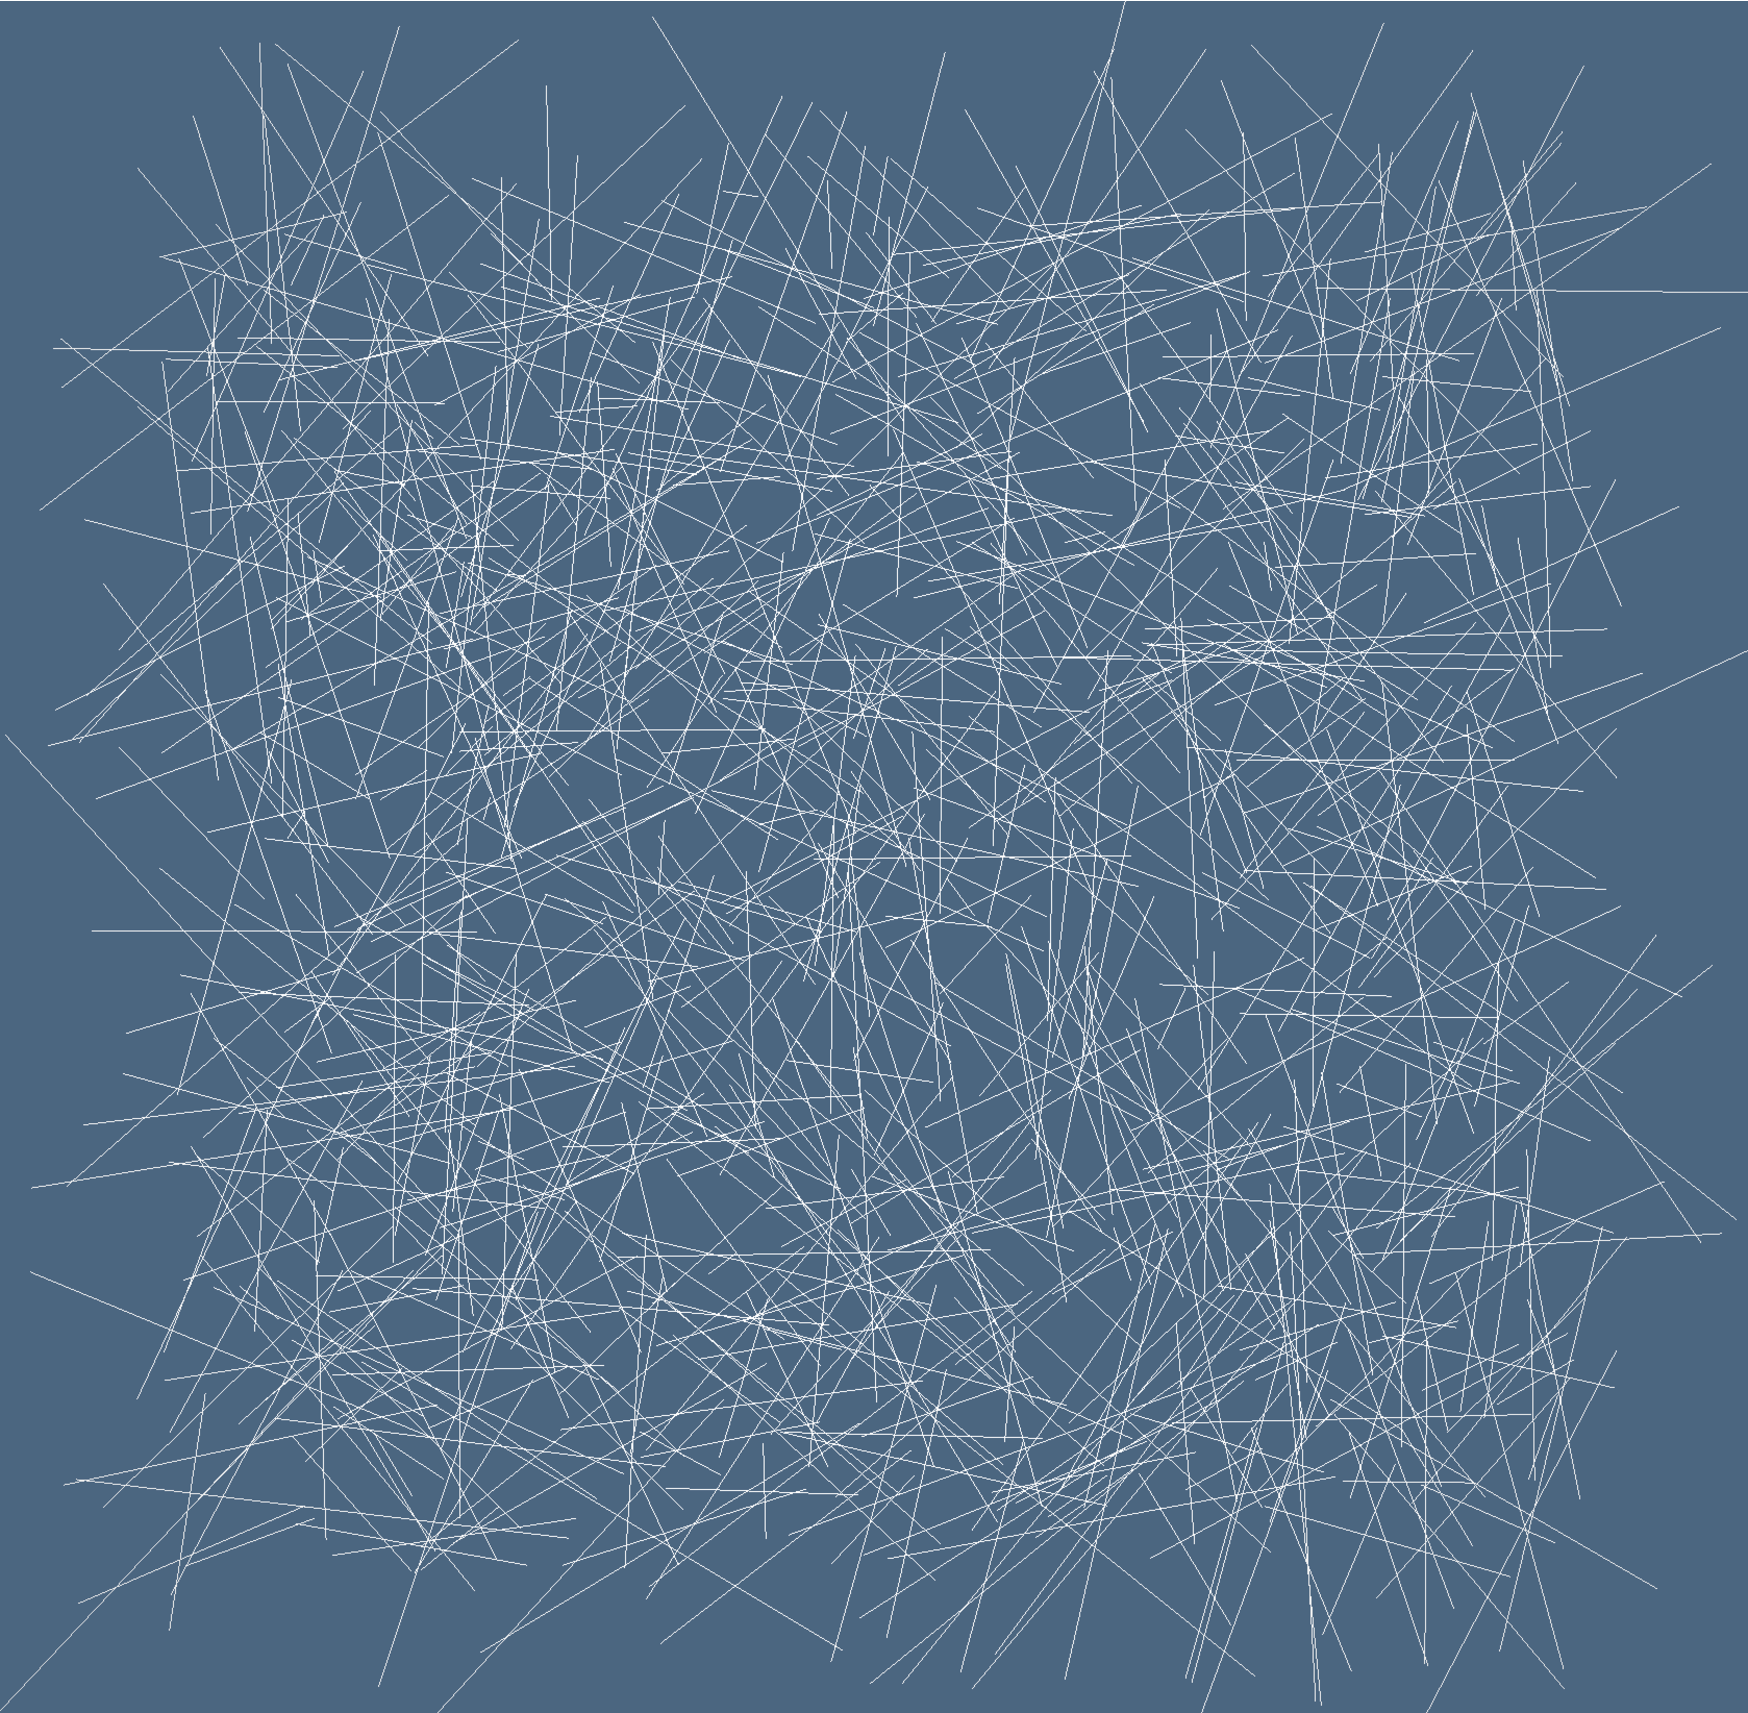
\includegraphics[height=0.495\textwidth,width=0.495\textwidth]{2Dcells-1} 
   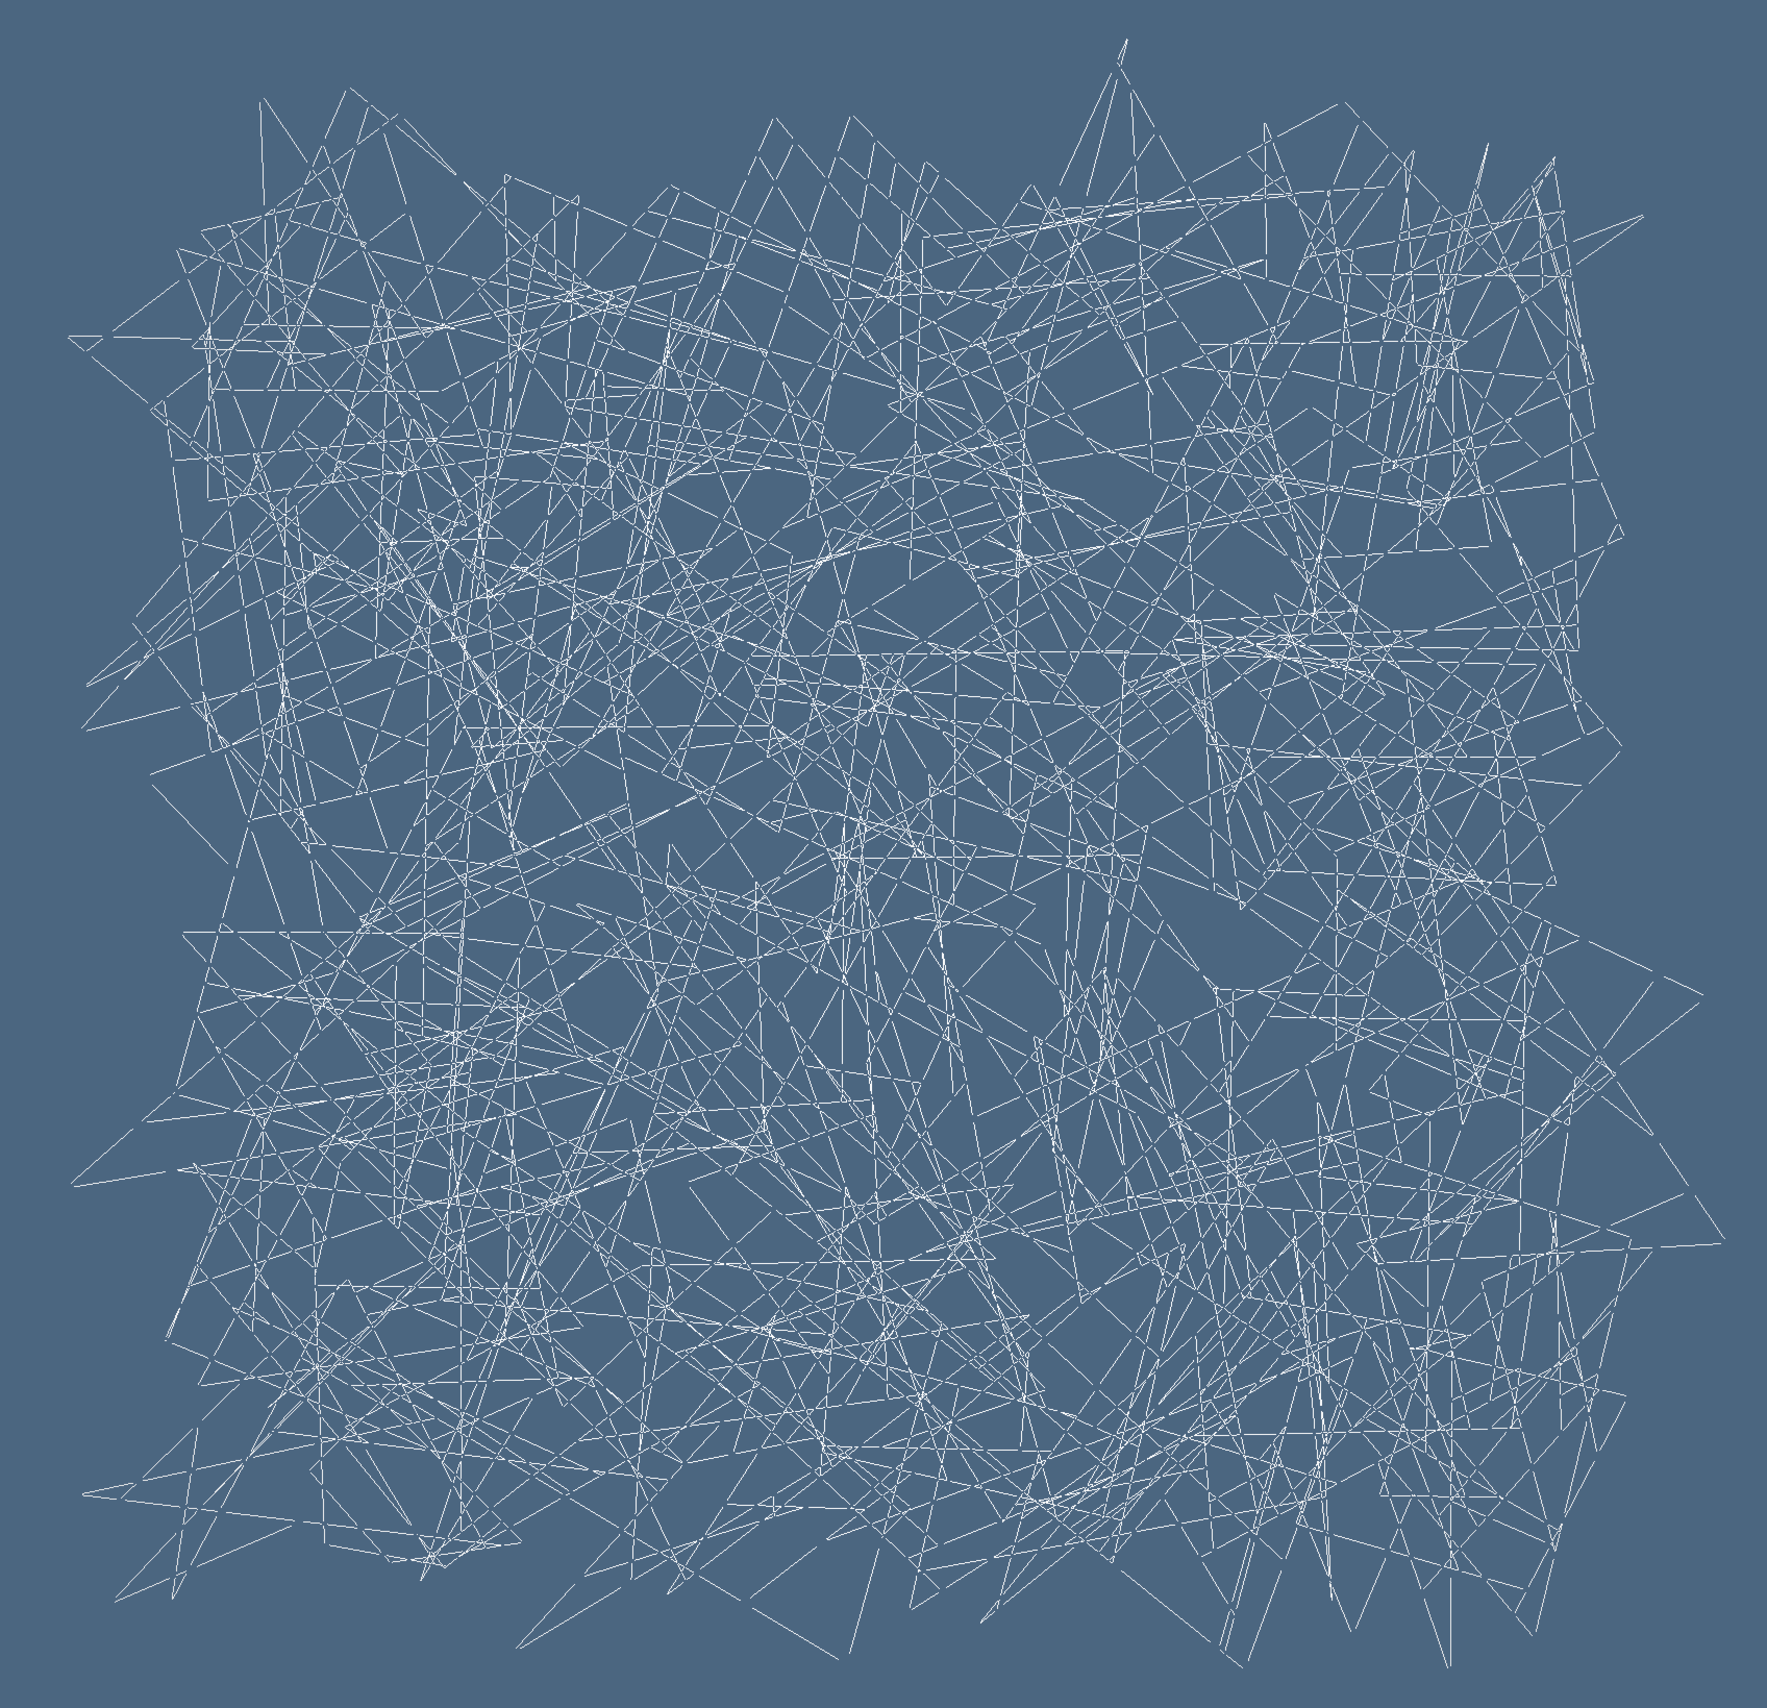
\includegraphics[height=0.495\textwidth,width=0.495\textwidth]{2Dcells-2} 
   
   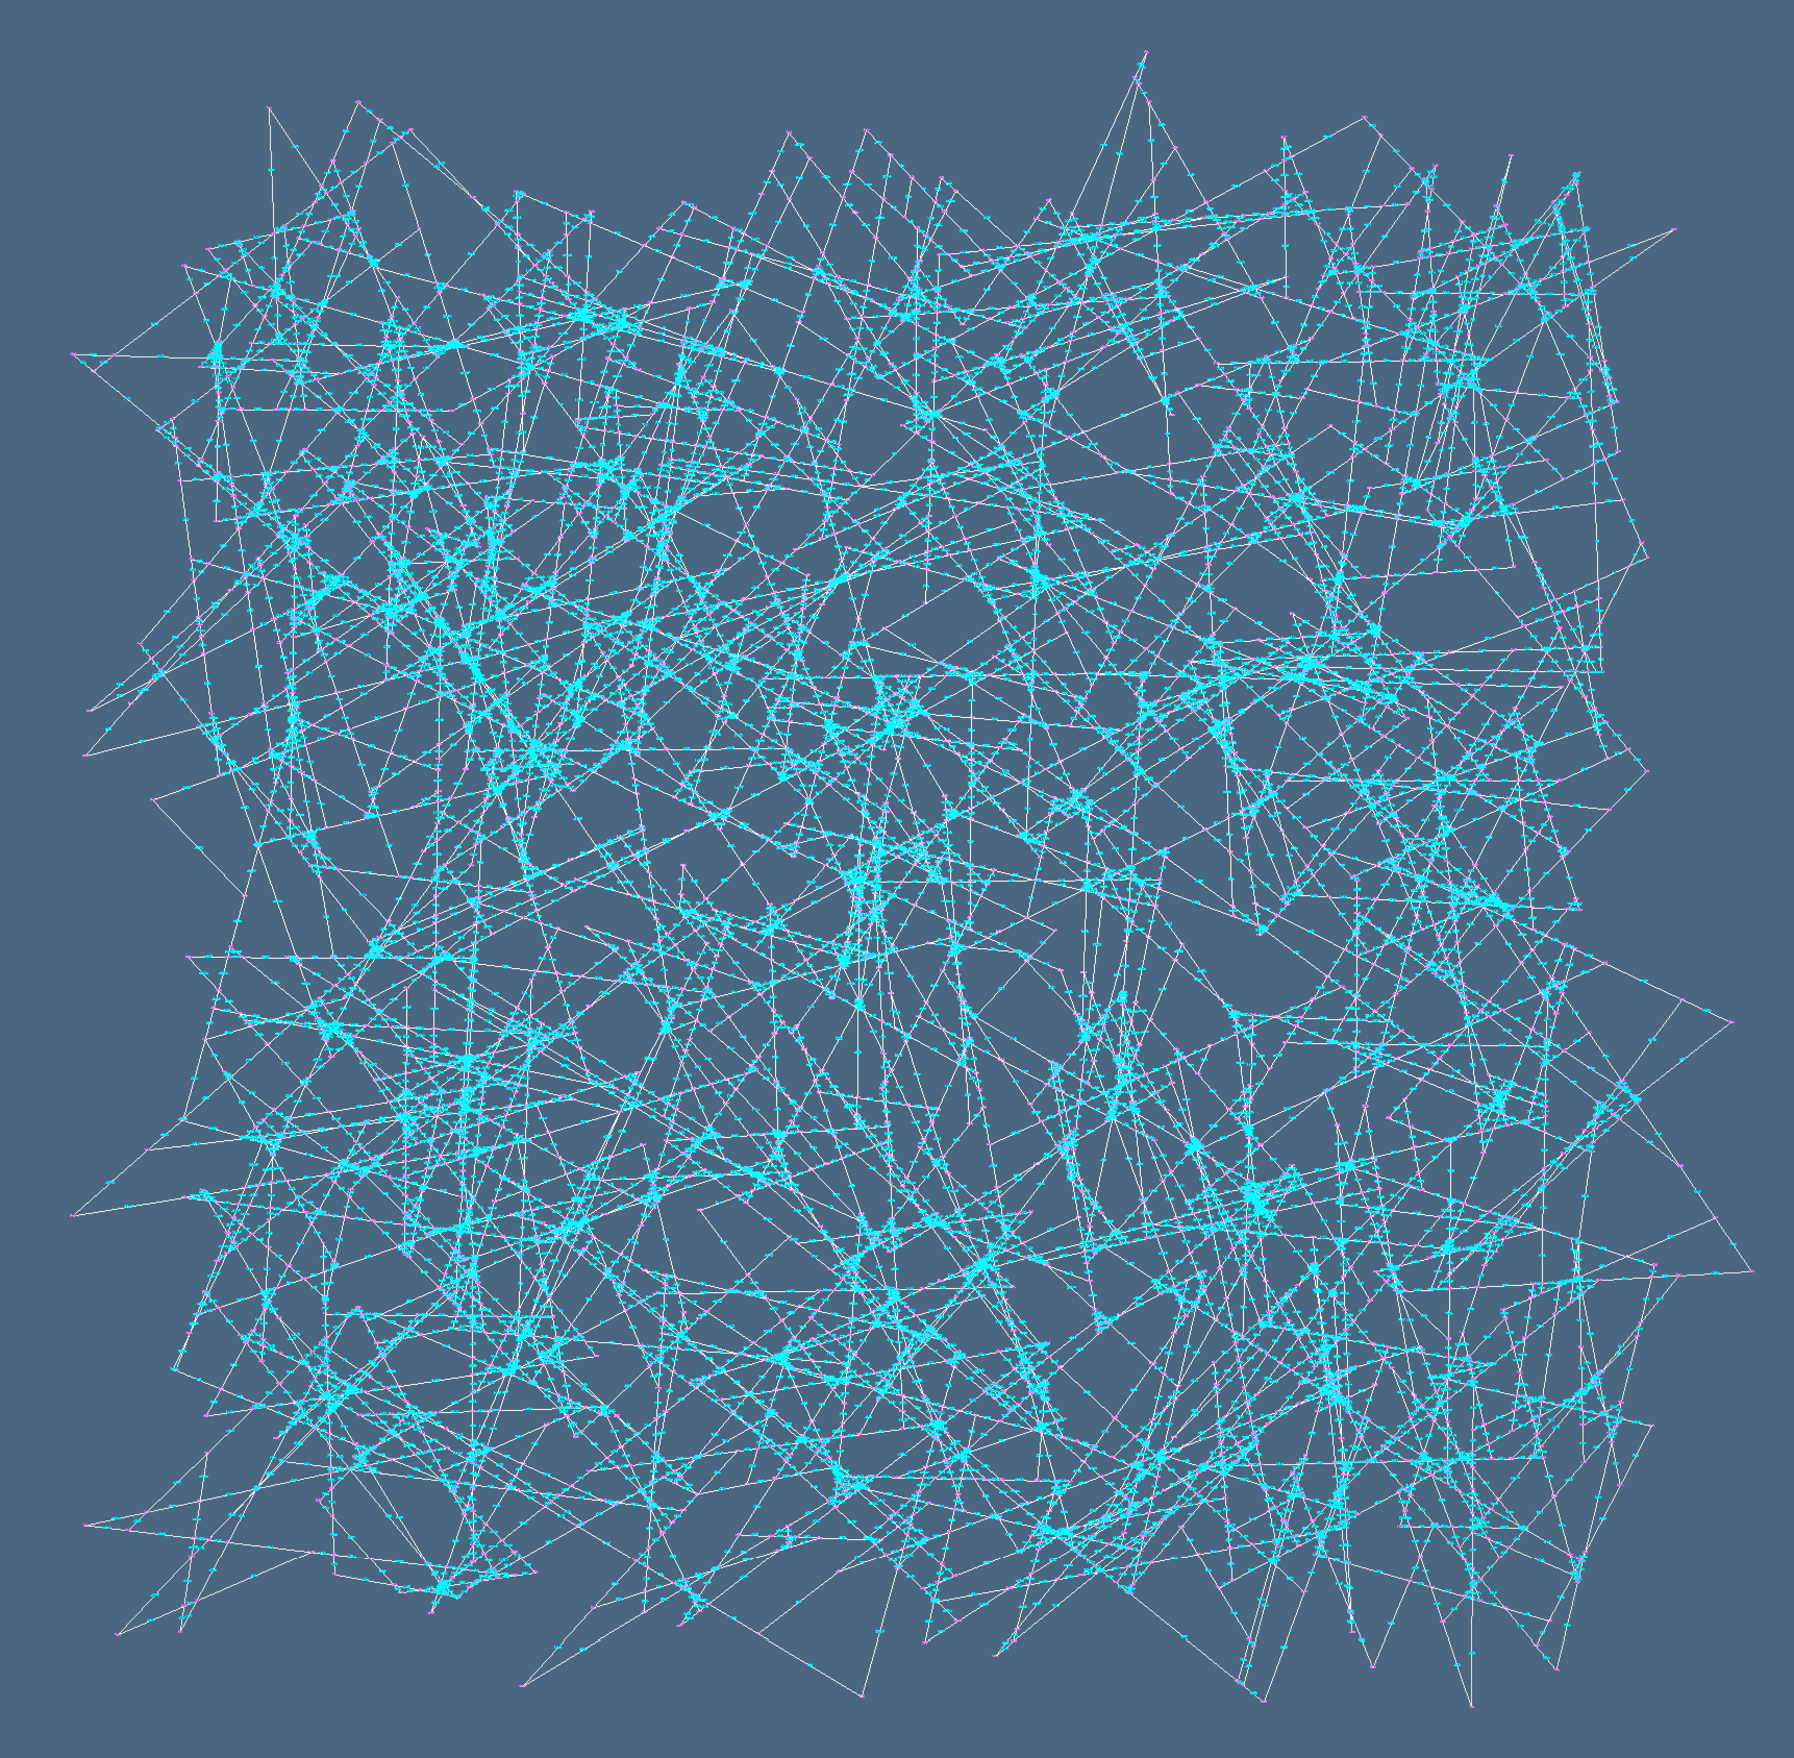
\includegraphics[height=0.495\textwidth,width=0.495\textwidth]{2Dcells-3} 
   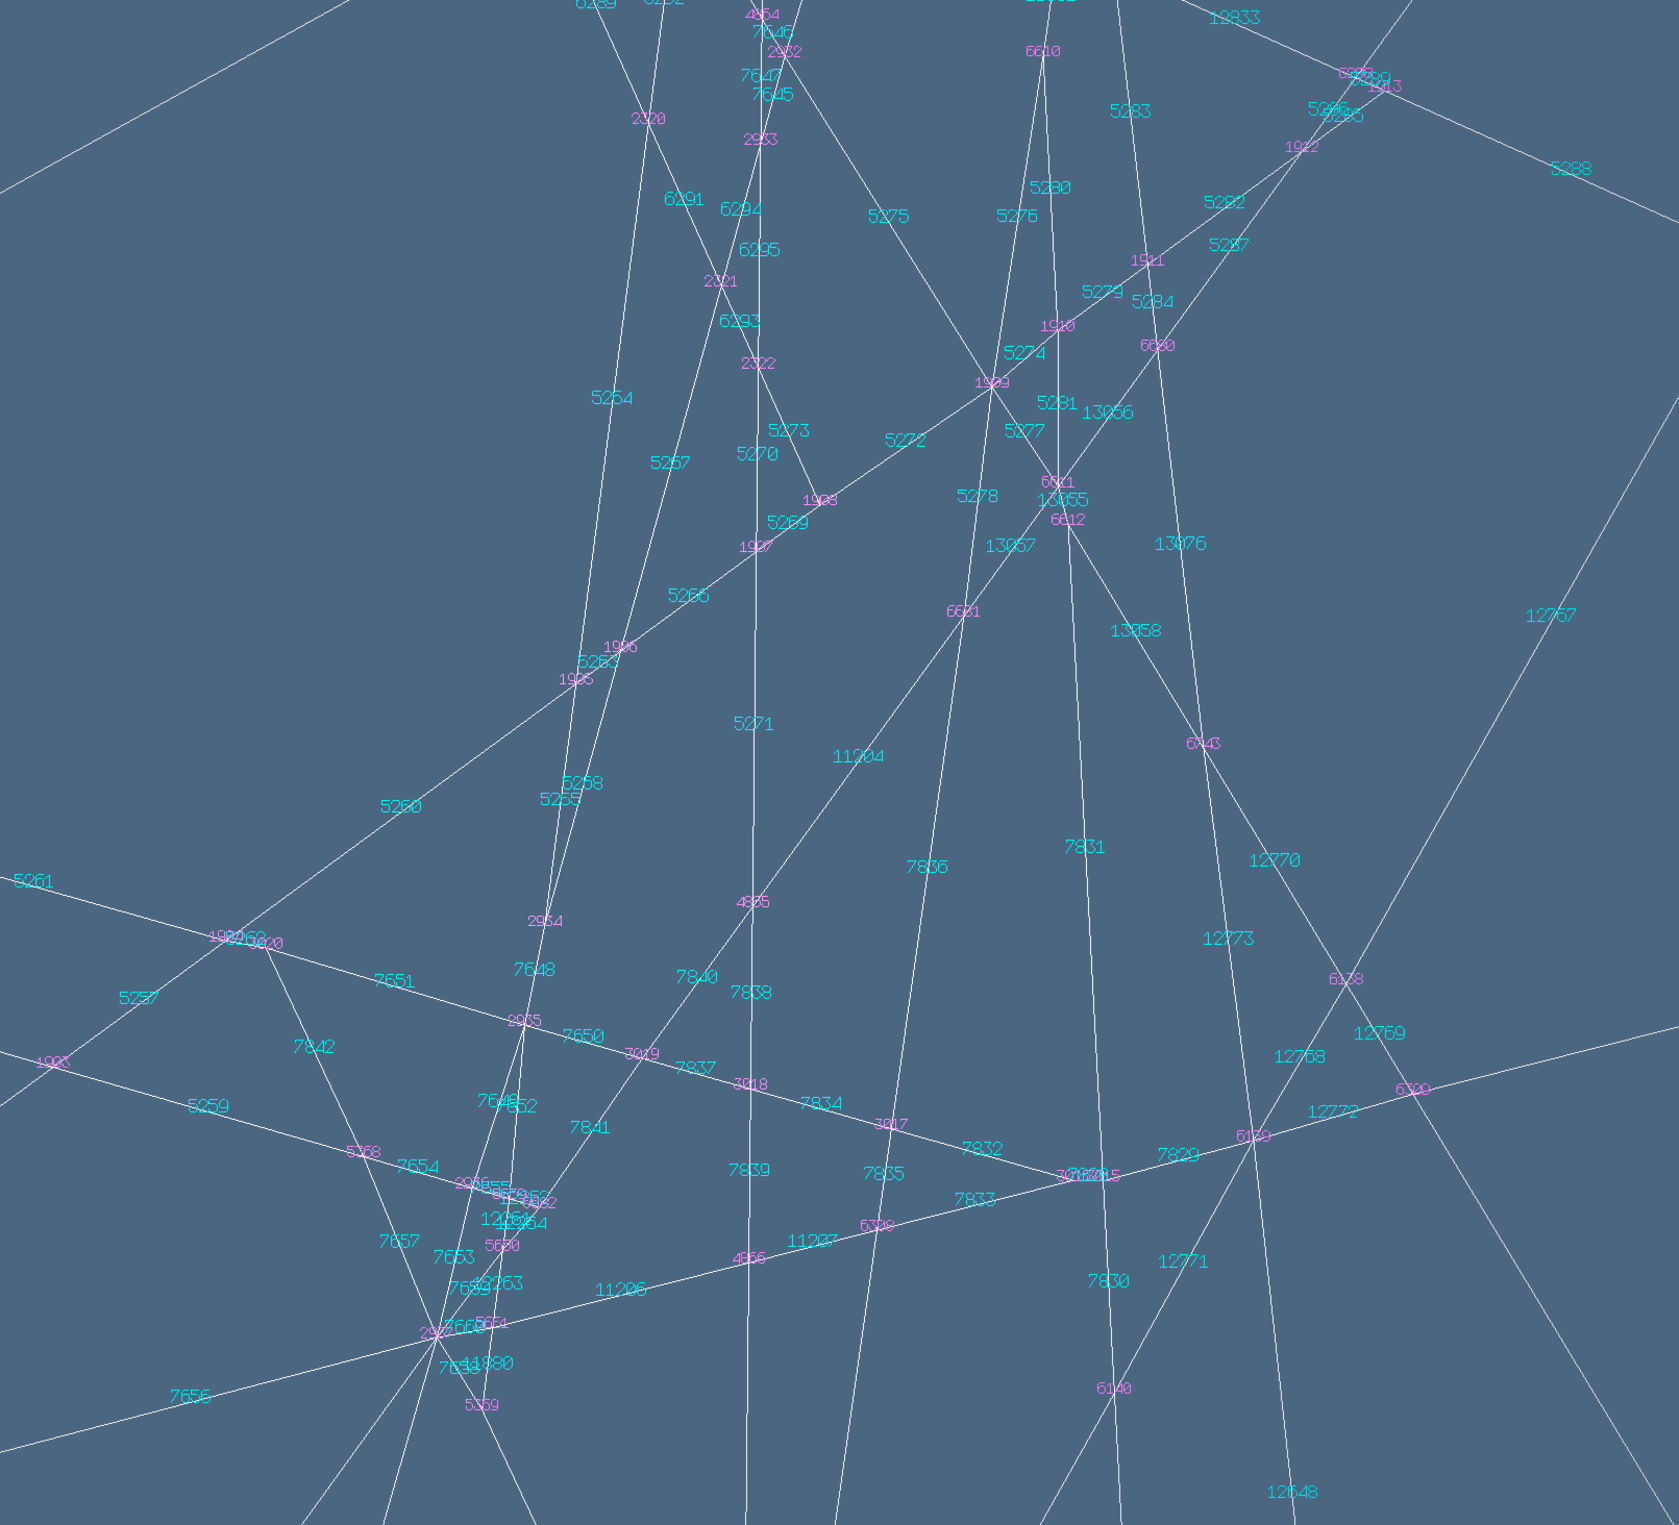
\includegraphics[height=0.495\textwidth,width=0.495\textwidth]{2Dcells-4} 

   \caption{The 2D regular(ized) complex generated by a random arrangement of lines:
   (a) the arrangement of lines; (b) the 2-connected subgraph of the divided lines; (c) the numbering of vertices and edges; (d) a close view of an arrangment portion. }
   \label{fig:2Dcells}
\end{figure}


\section{Planimetric 2-complex}

Here it is shown both the input and the output of the simplest example of architectural data. The same approach would holds for cartographics applications at any scale (see Figures~\ref{fig:rectangles} and~\ref{fig:testWall}).

\begin{figure}[htbp] %  figure placement: here, top, bottom, or page
   \centering
   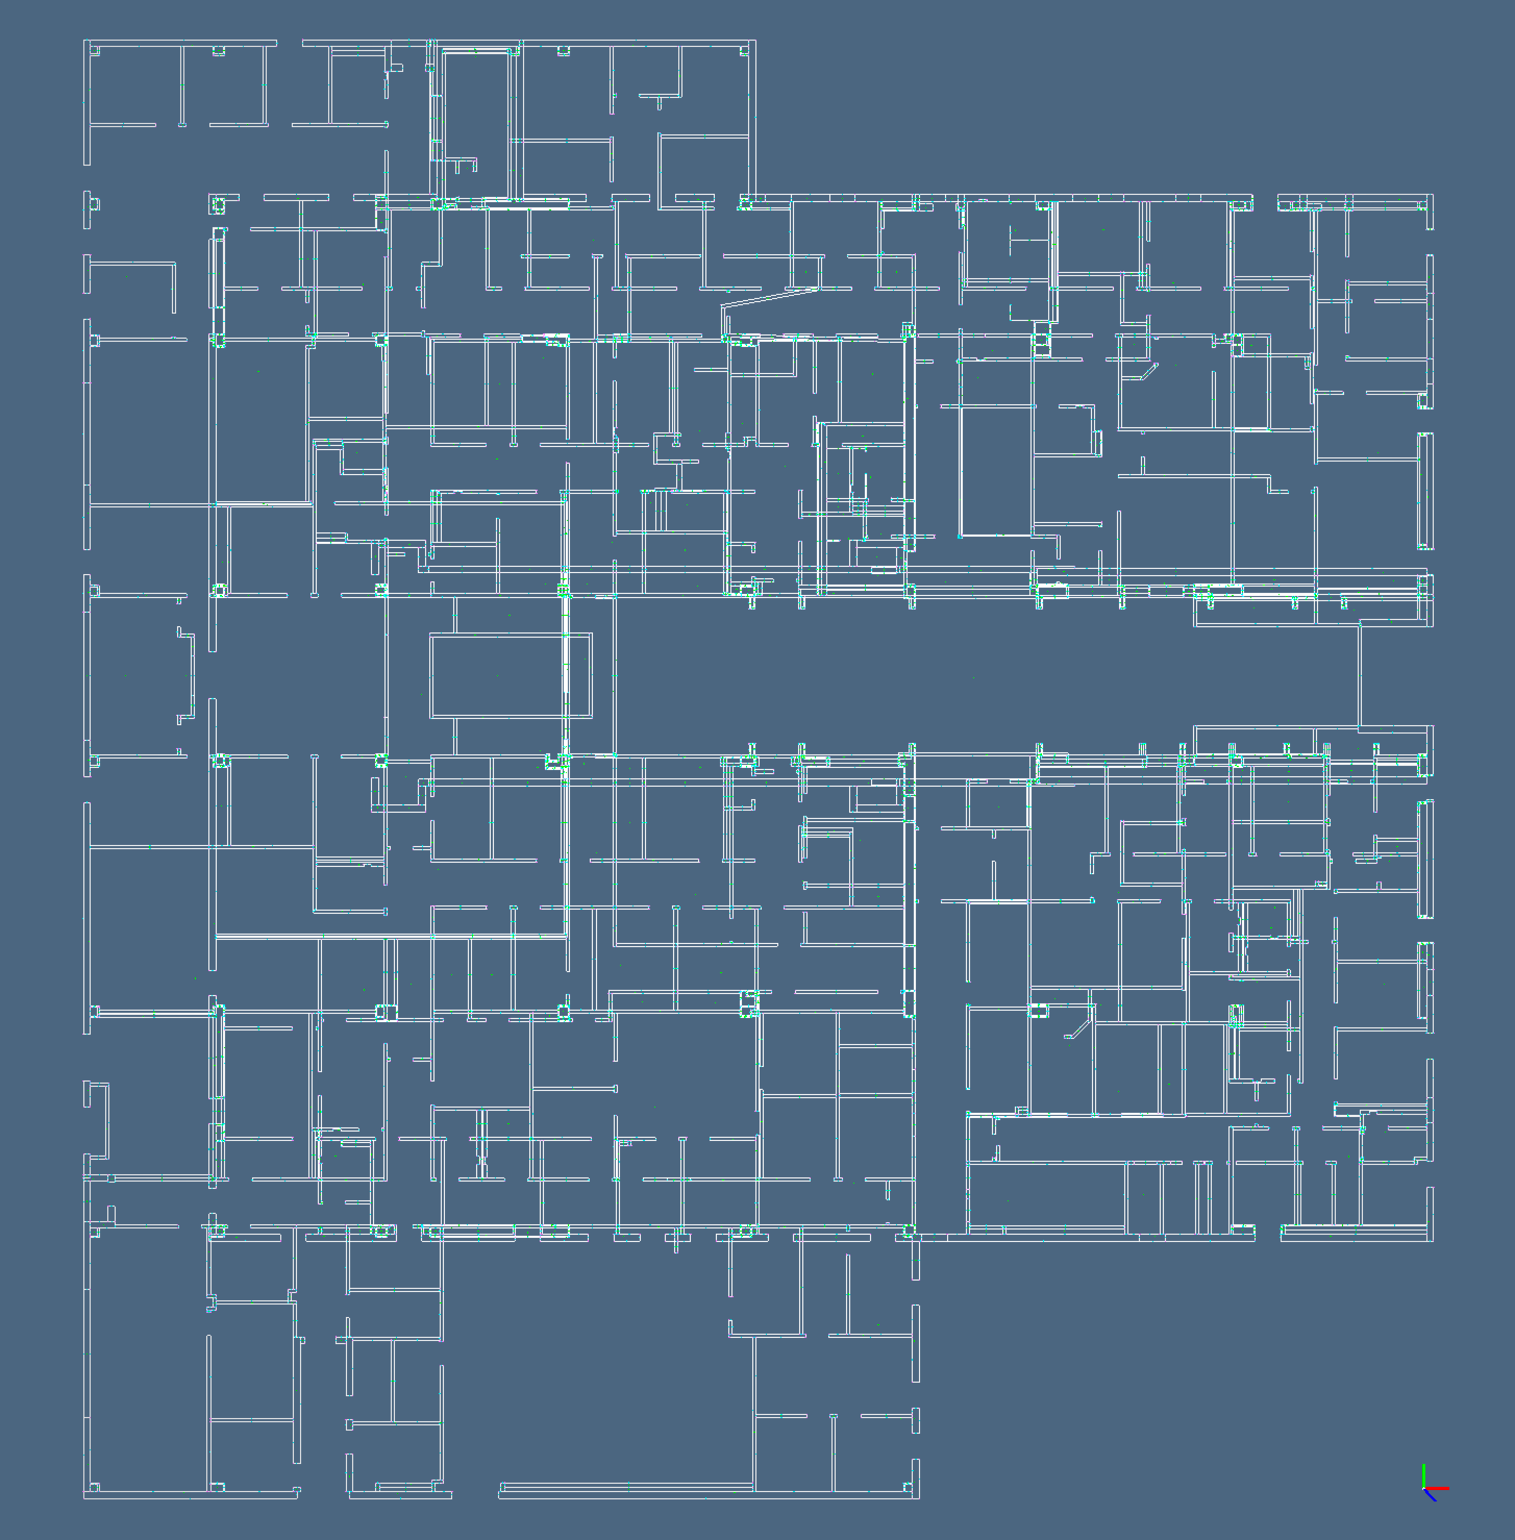
\includegraphics[width=0.44\textwidth]{testWall1} 
   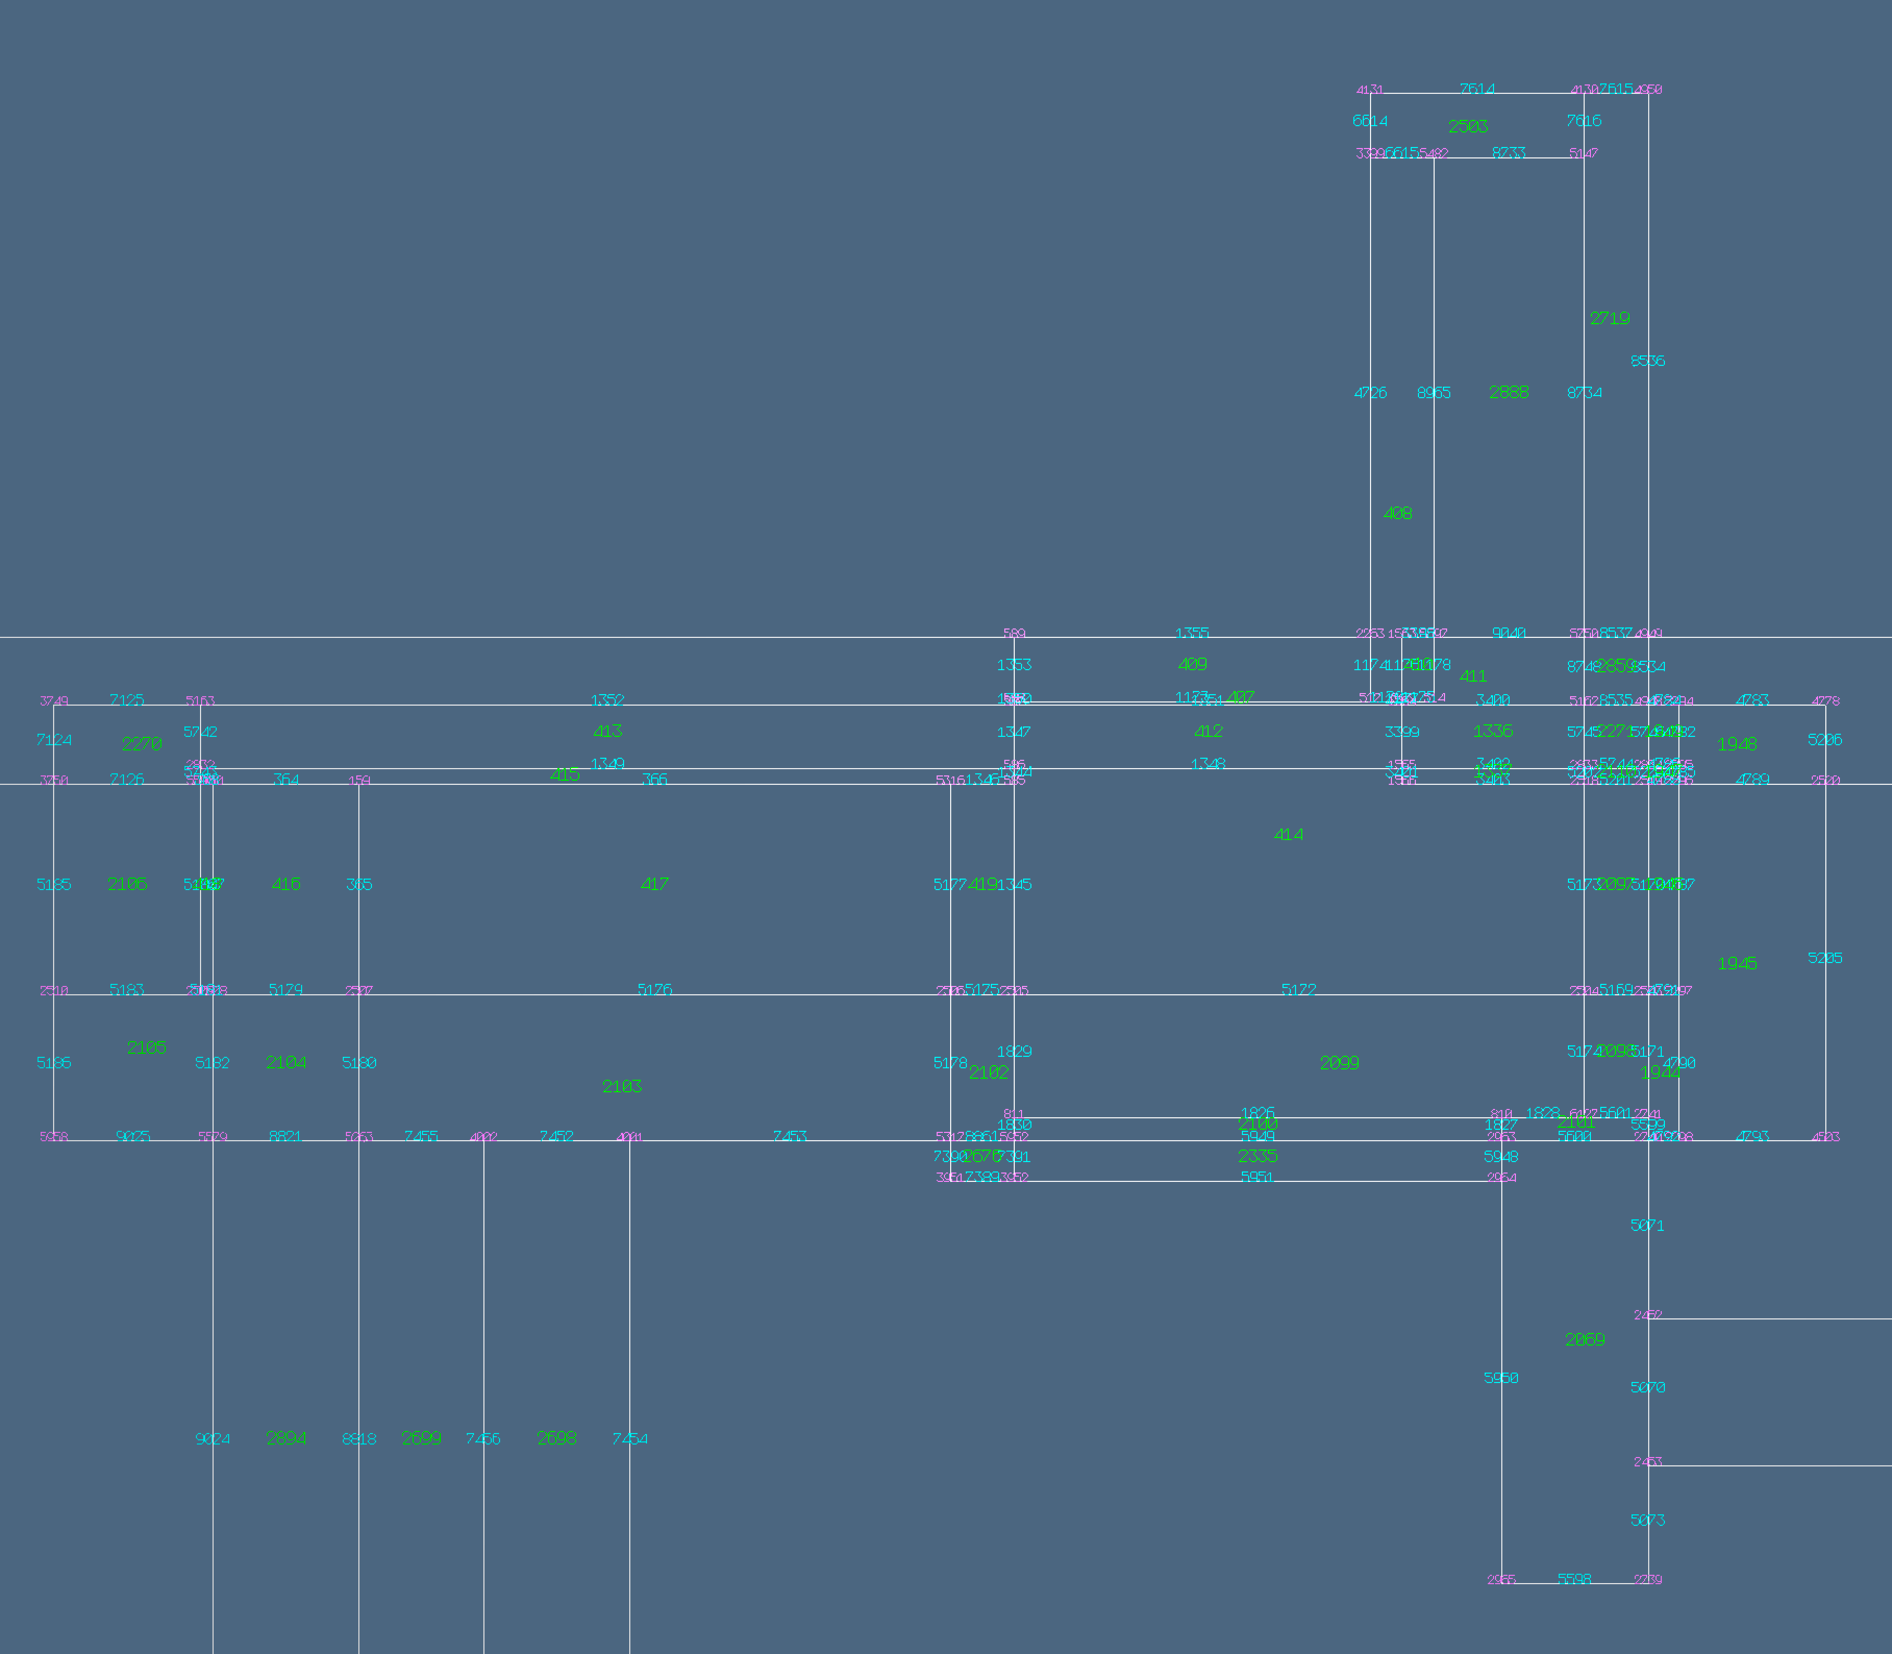
\includegraphics[width=0.51\textwidth]{testWall2} 
   \caption{.}
   \label{fig:testWall}
\end{figure}

\subsection{Input data}

The input

\begin{figure}[htbp] %  figure placement: here, top, bottom, or page
   \centering
   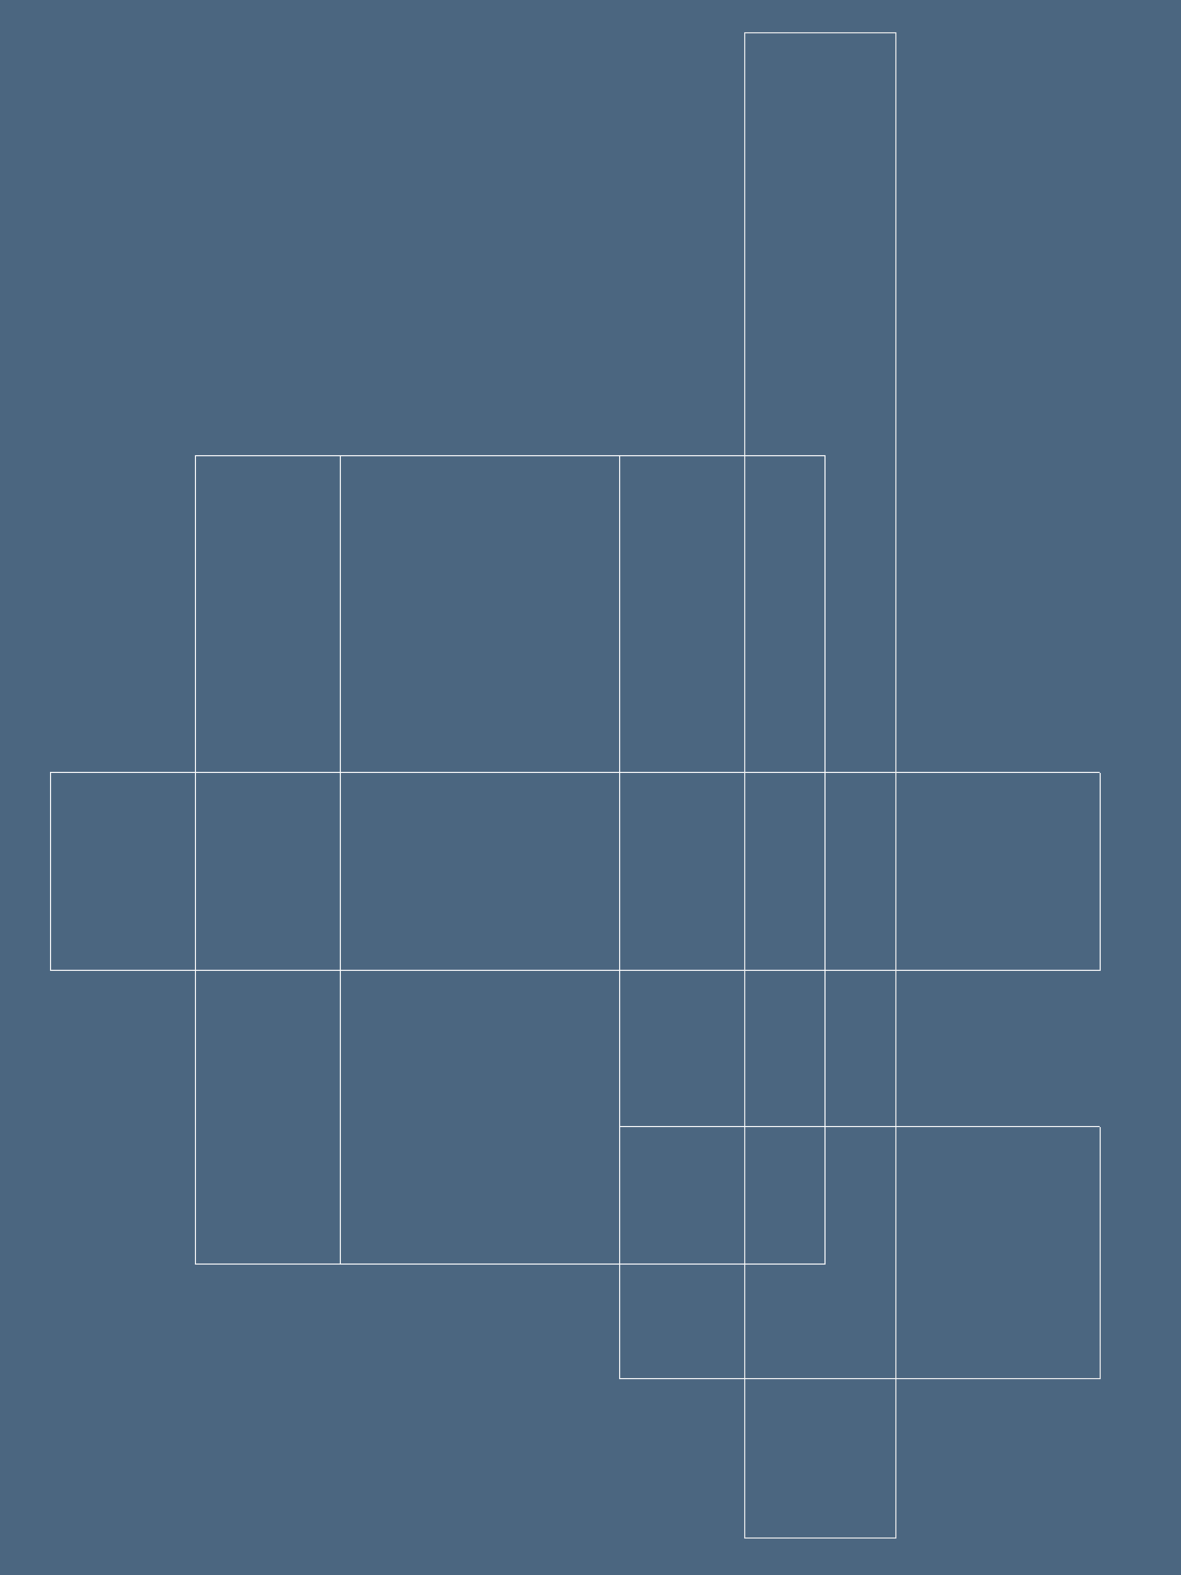
\includegraphics[width=0.4\textwidth]{rectangles0} 
   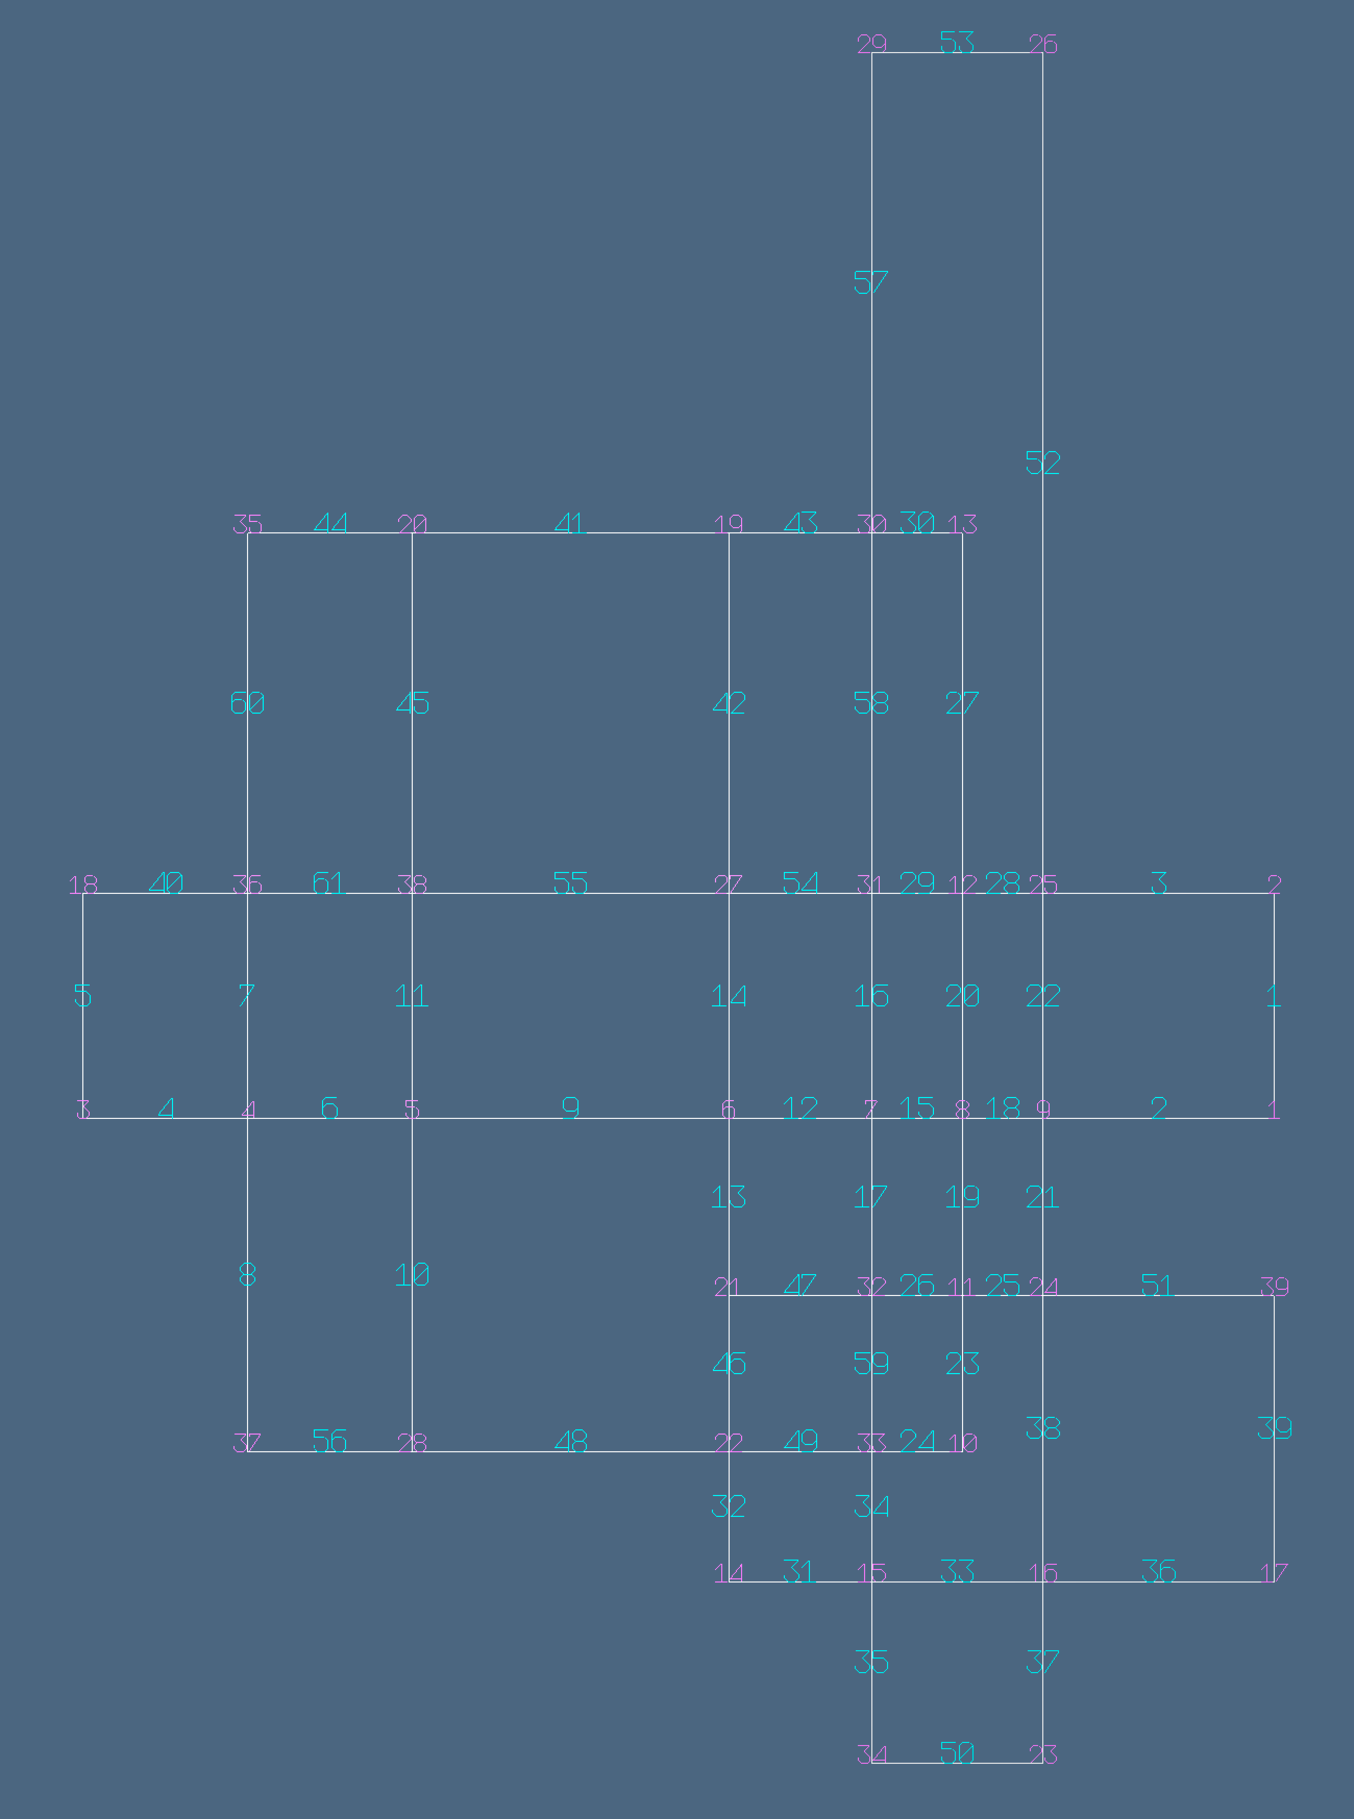
\includegraphics[width=0.4\textwidth]{rectangles1} 
   
   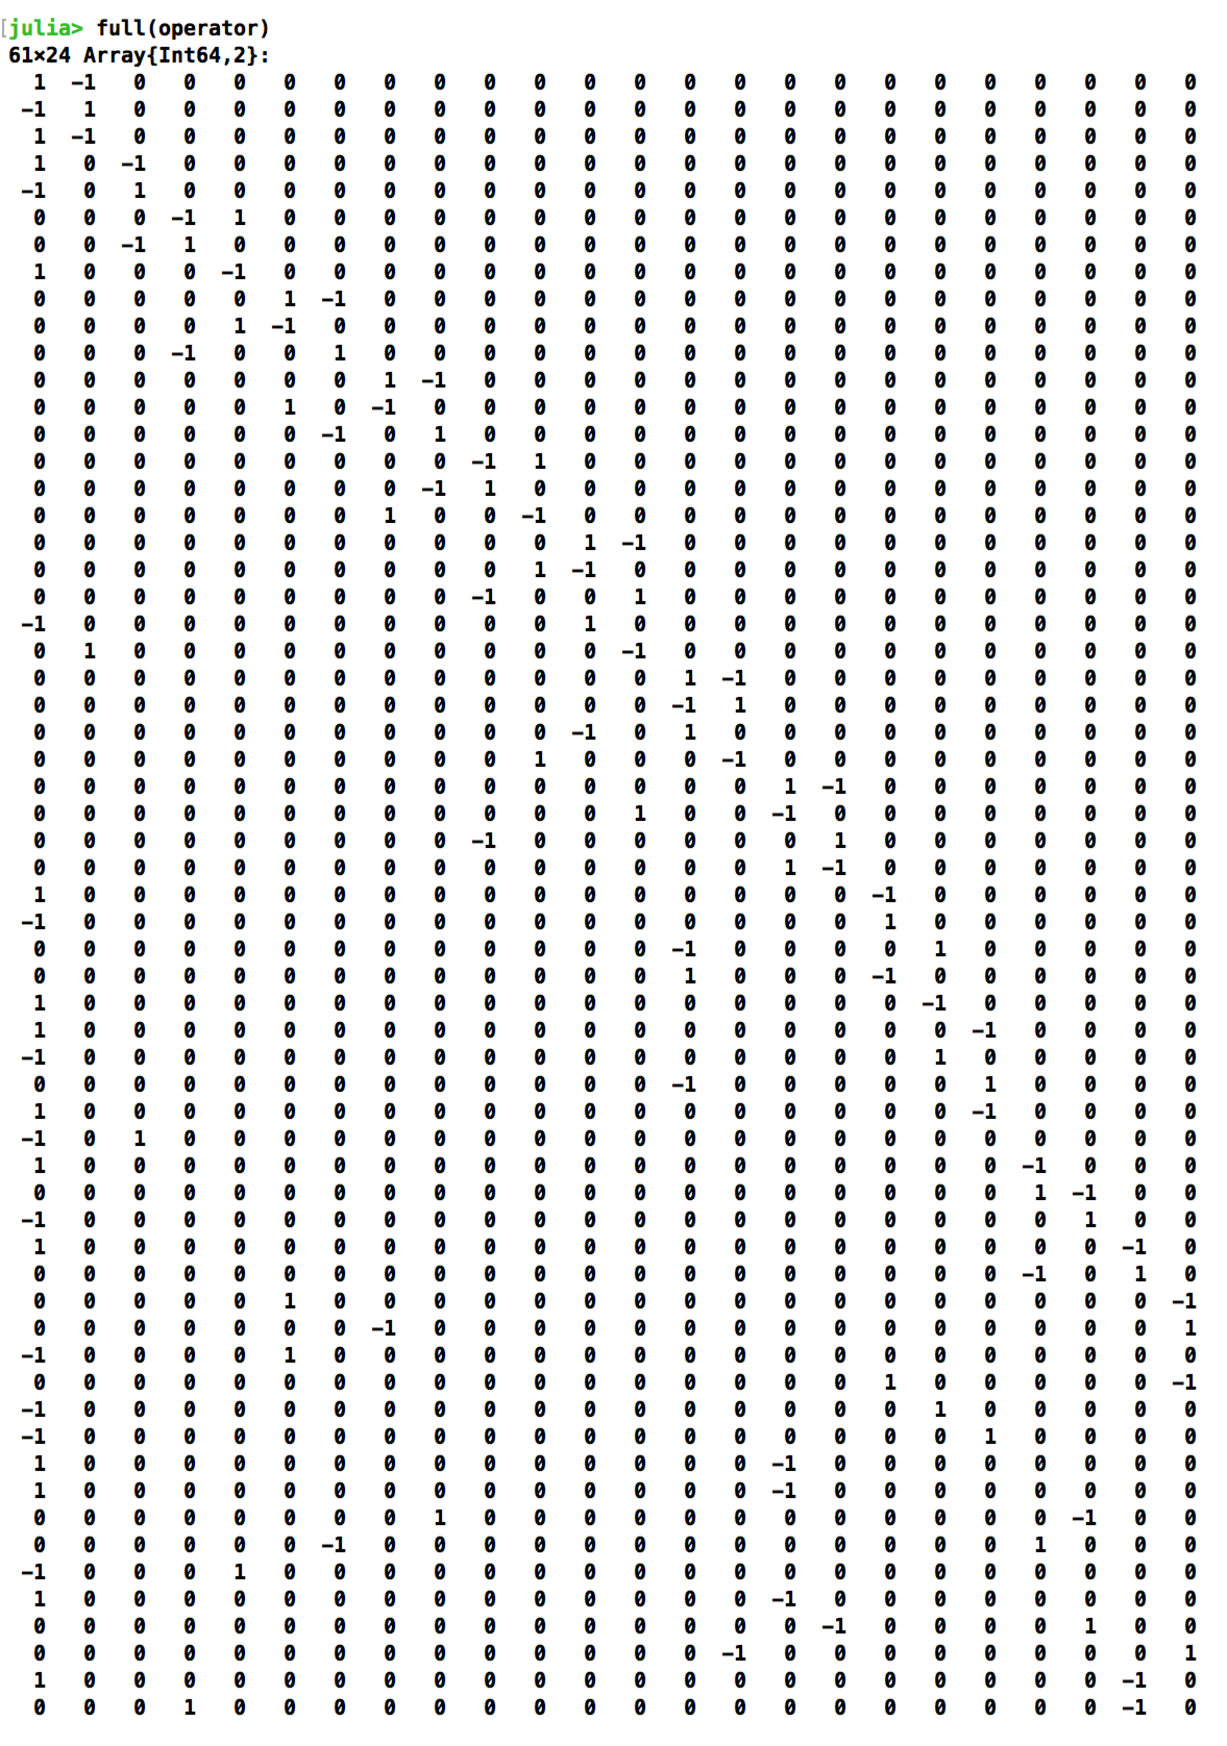
\includegraphics[width=0.4\textwidth]{rectangles2} 
   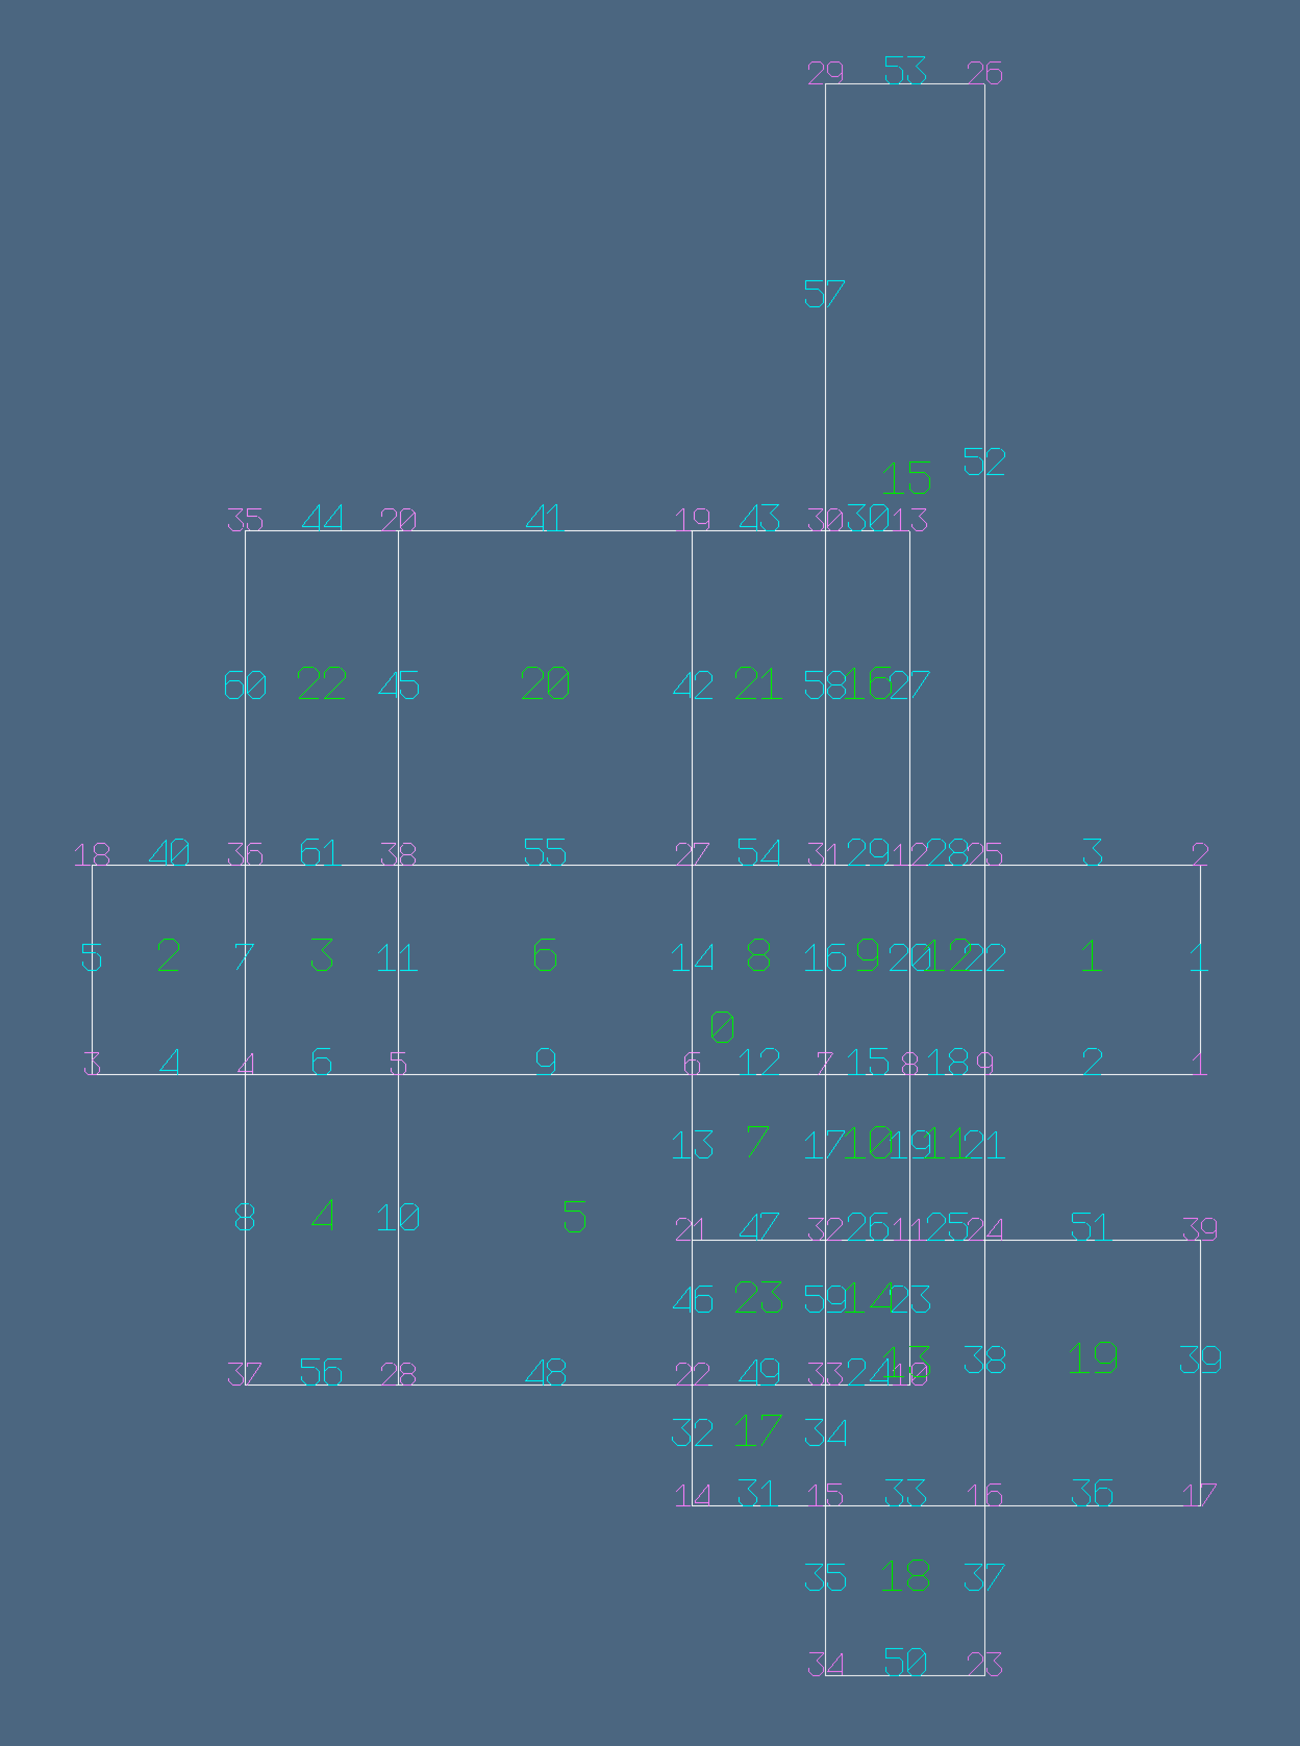
\includegraphics[width=0.4\textwidth]{rectangles3} 
   \caption{Cellular 2-complex built starting from a set of lines. (a) the input data, i.e.~partially or totally superimposed lines; (b) 1-complex after line intersections; (c) matrix of $\partial_2$ operator; (d) 2-complex produced by LAR calculi.}
   \label{fig:rectangles}
\end{figure}



\begin{figure}[htbp] %  figure placement: here, top, bottom, or page
   \centering
   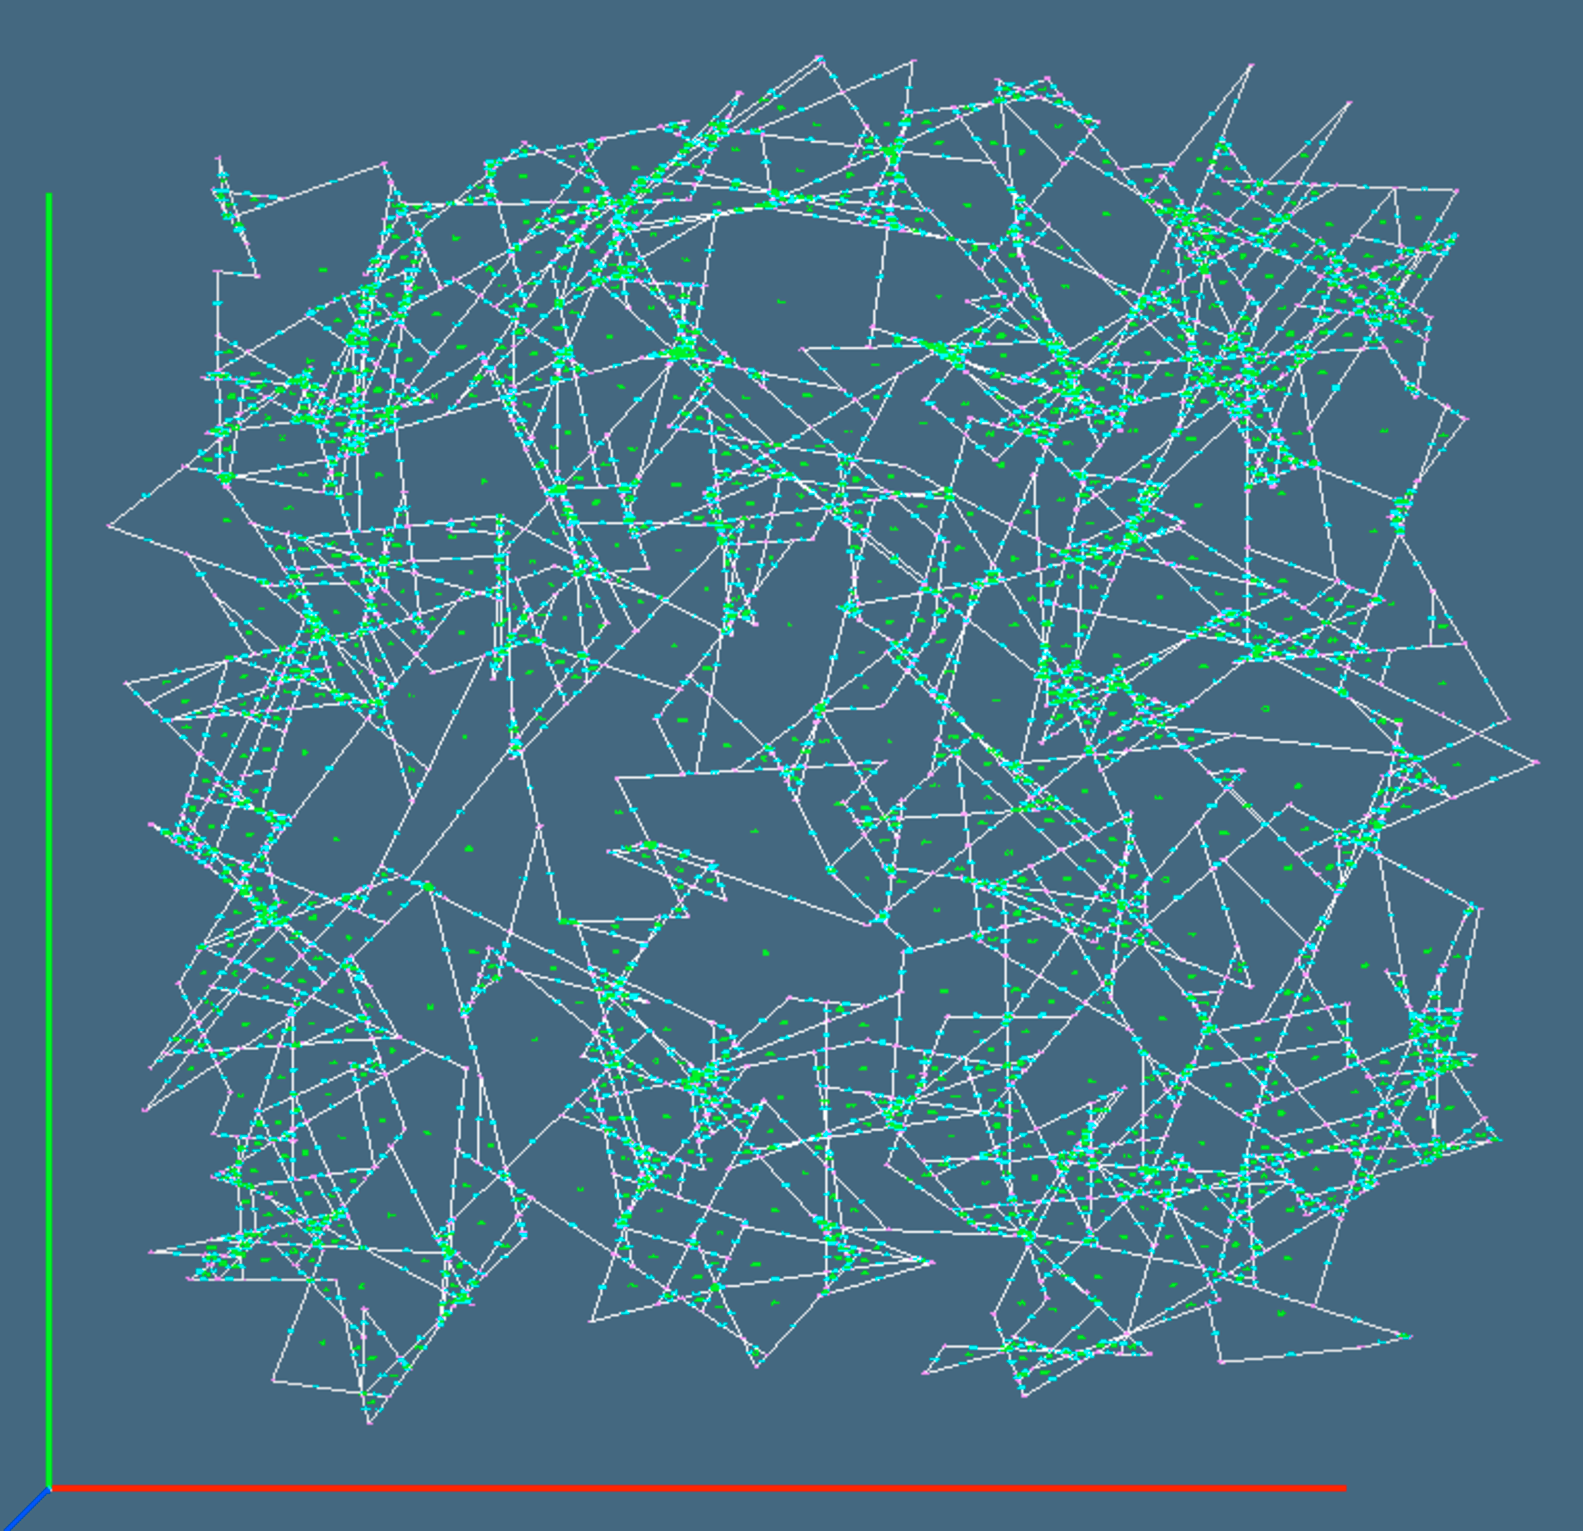
\includegraphics[width=0.328\textheight,width=0.328\textwidth]{2dcells0} 
   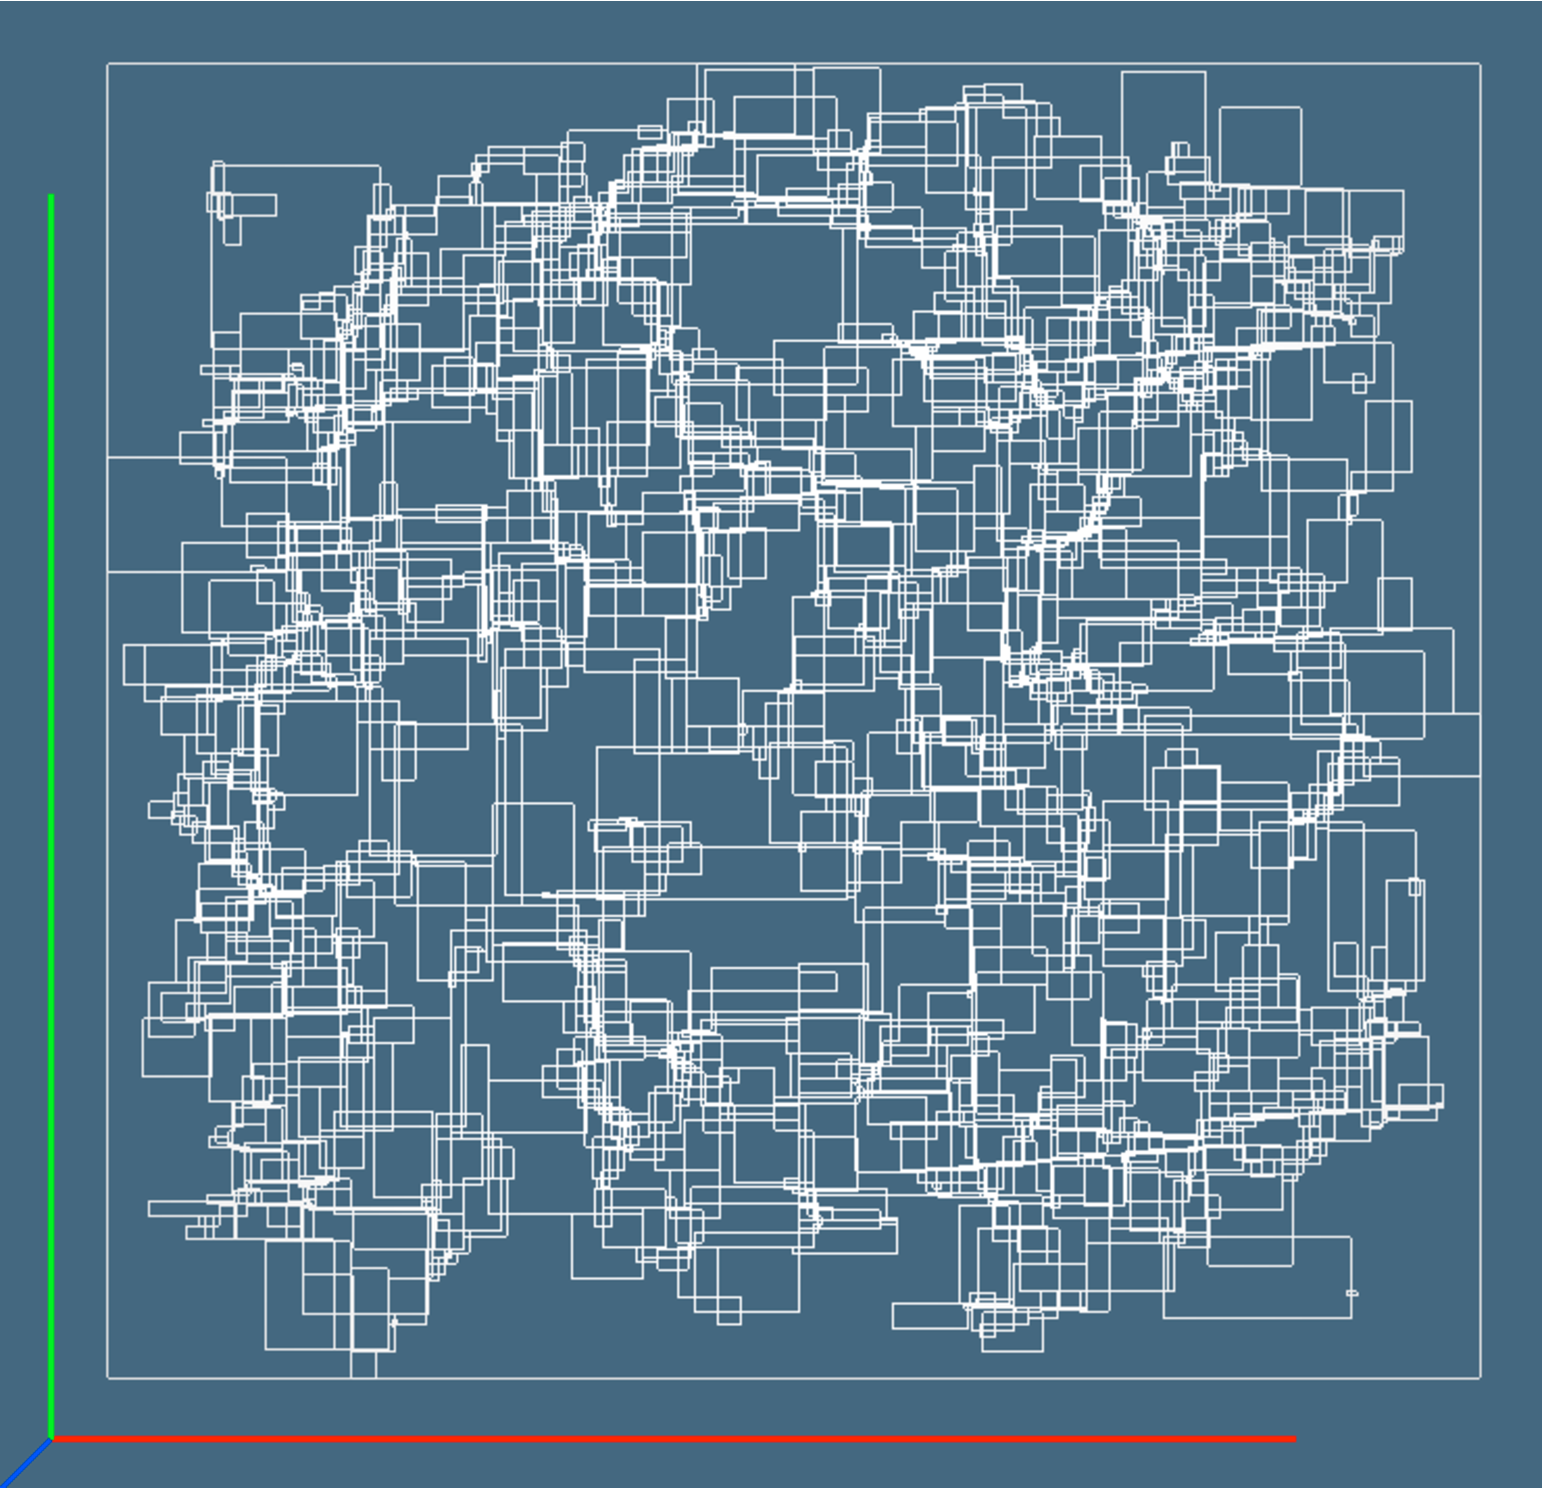
\includegraphics[width=0.328\textheight,width=0.328\textwidth]{2dcells1} 
   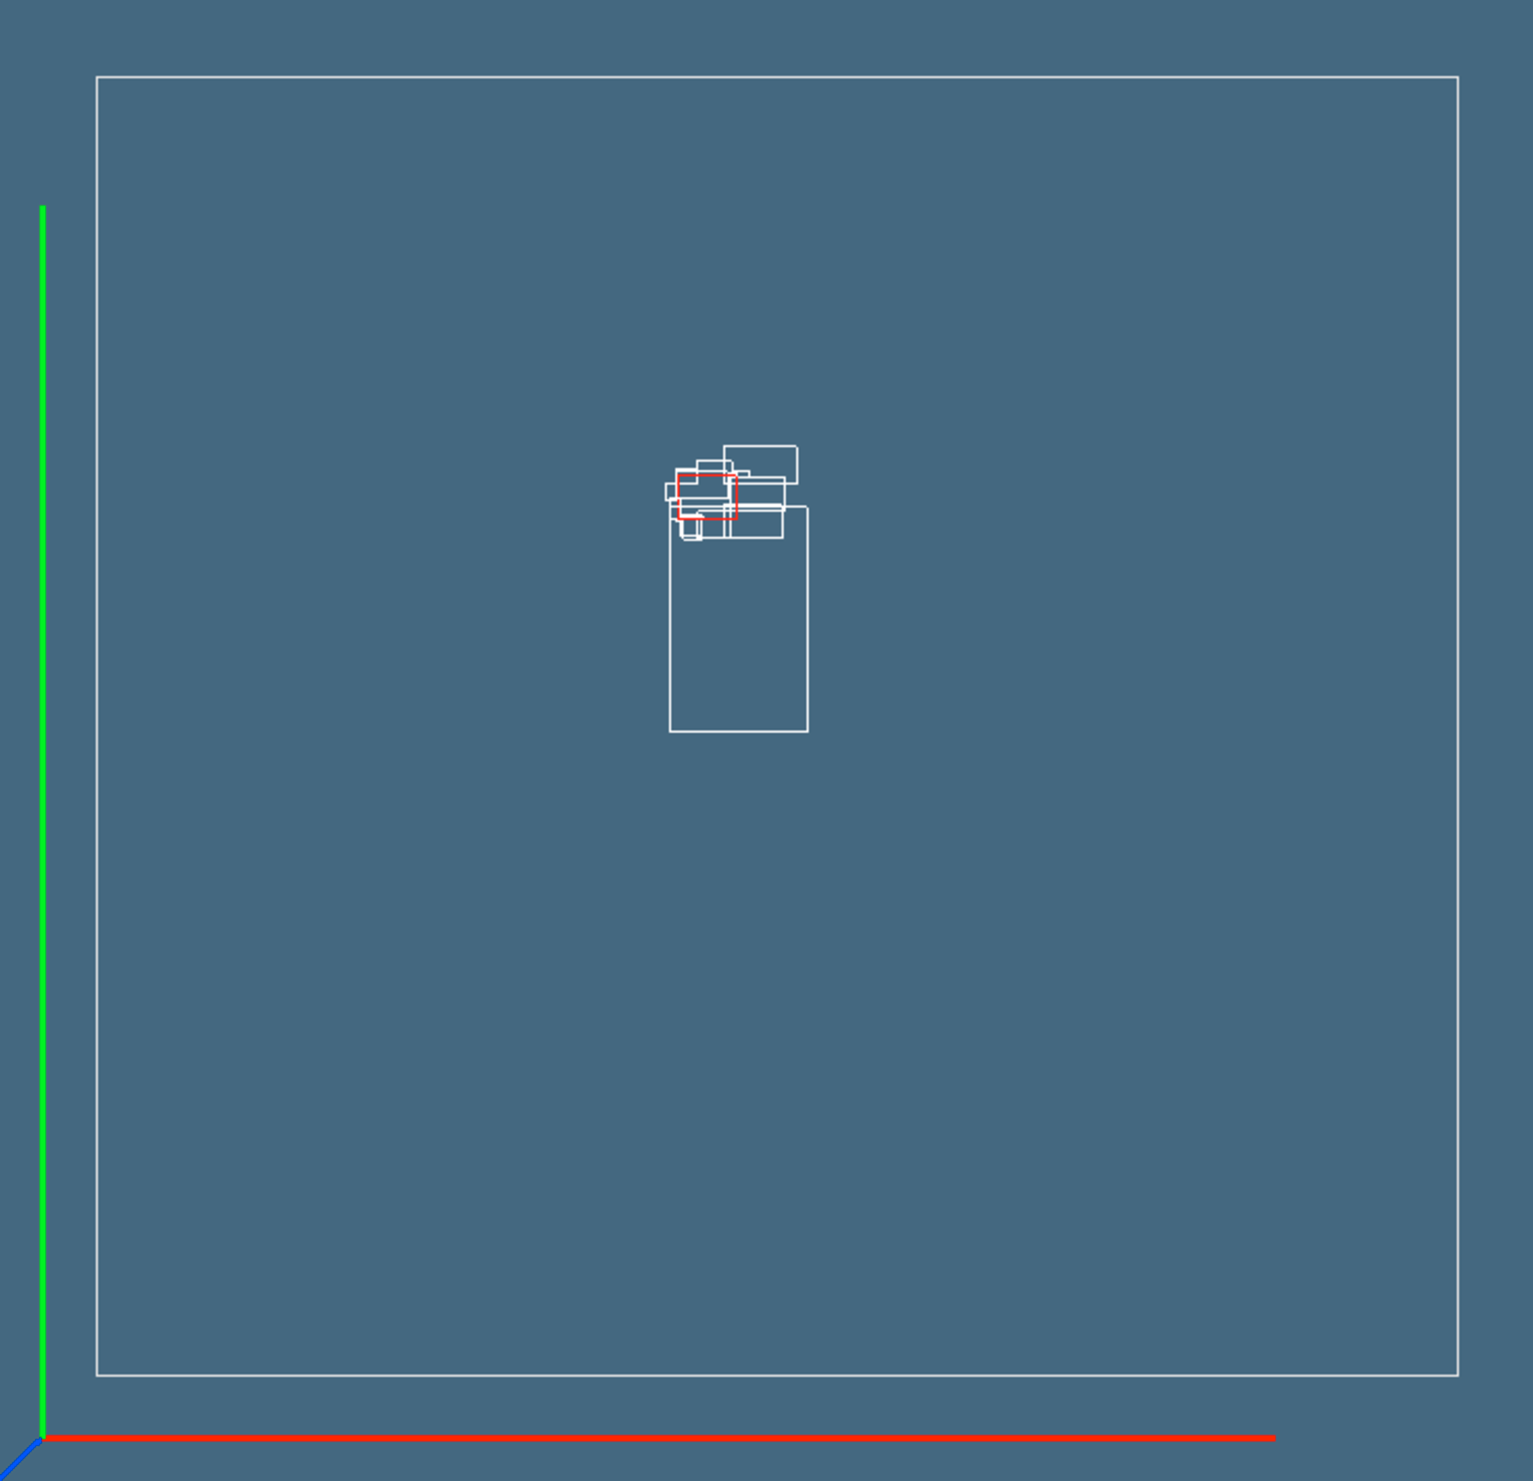
\includegraphics[width=0.328\textheight,width=0.328\textwidth]{2dcells2} 
   \caption{Fast intersection query of containment boxes od 2-cells using Interval Trees: (a) a random 2D decomposition generated by an arrangment of lines; (b) the containment boxes of all 2-cells; (c)  the result of an intersection query with the red box.}
   \label{fig:testWall}
\end{figure}



\begin{figure}[htbp] %  figure placement: here, top, bottom, or page
   \centering
   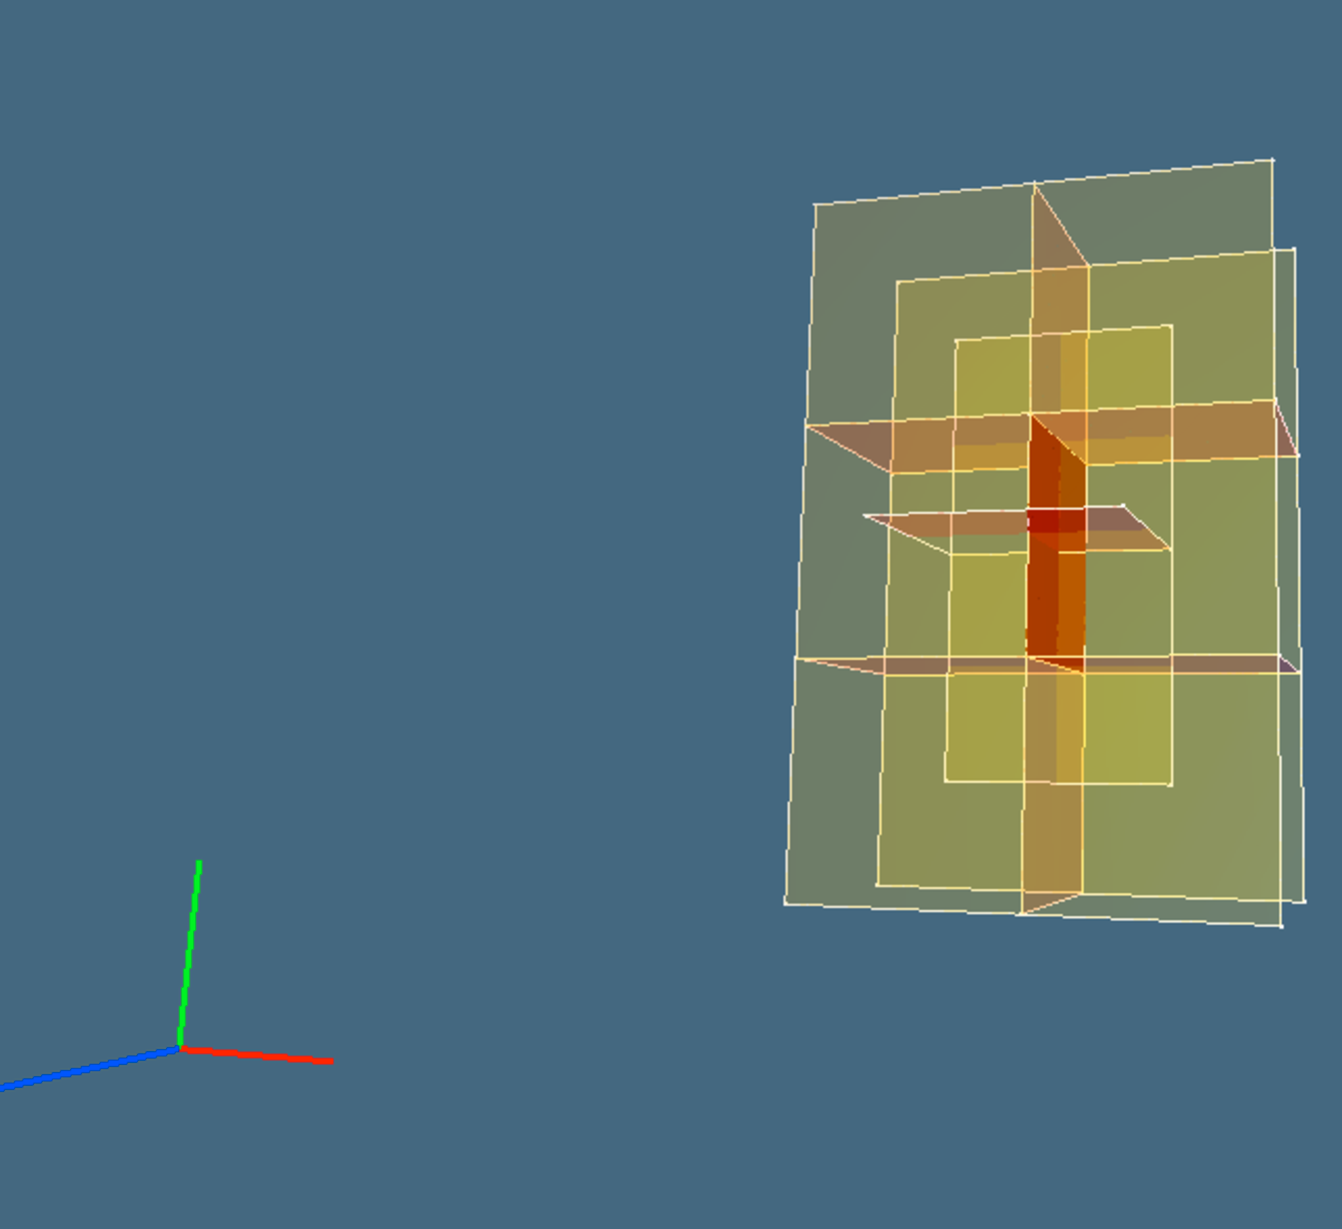
\includegraphics[width=0.5\textheight,width=0.51\textwidth]{submanifold1} 
   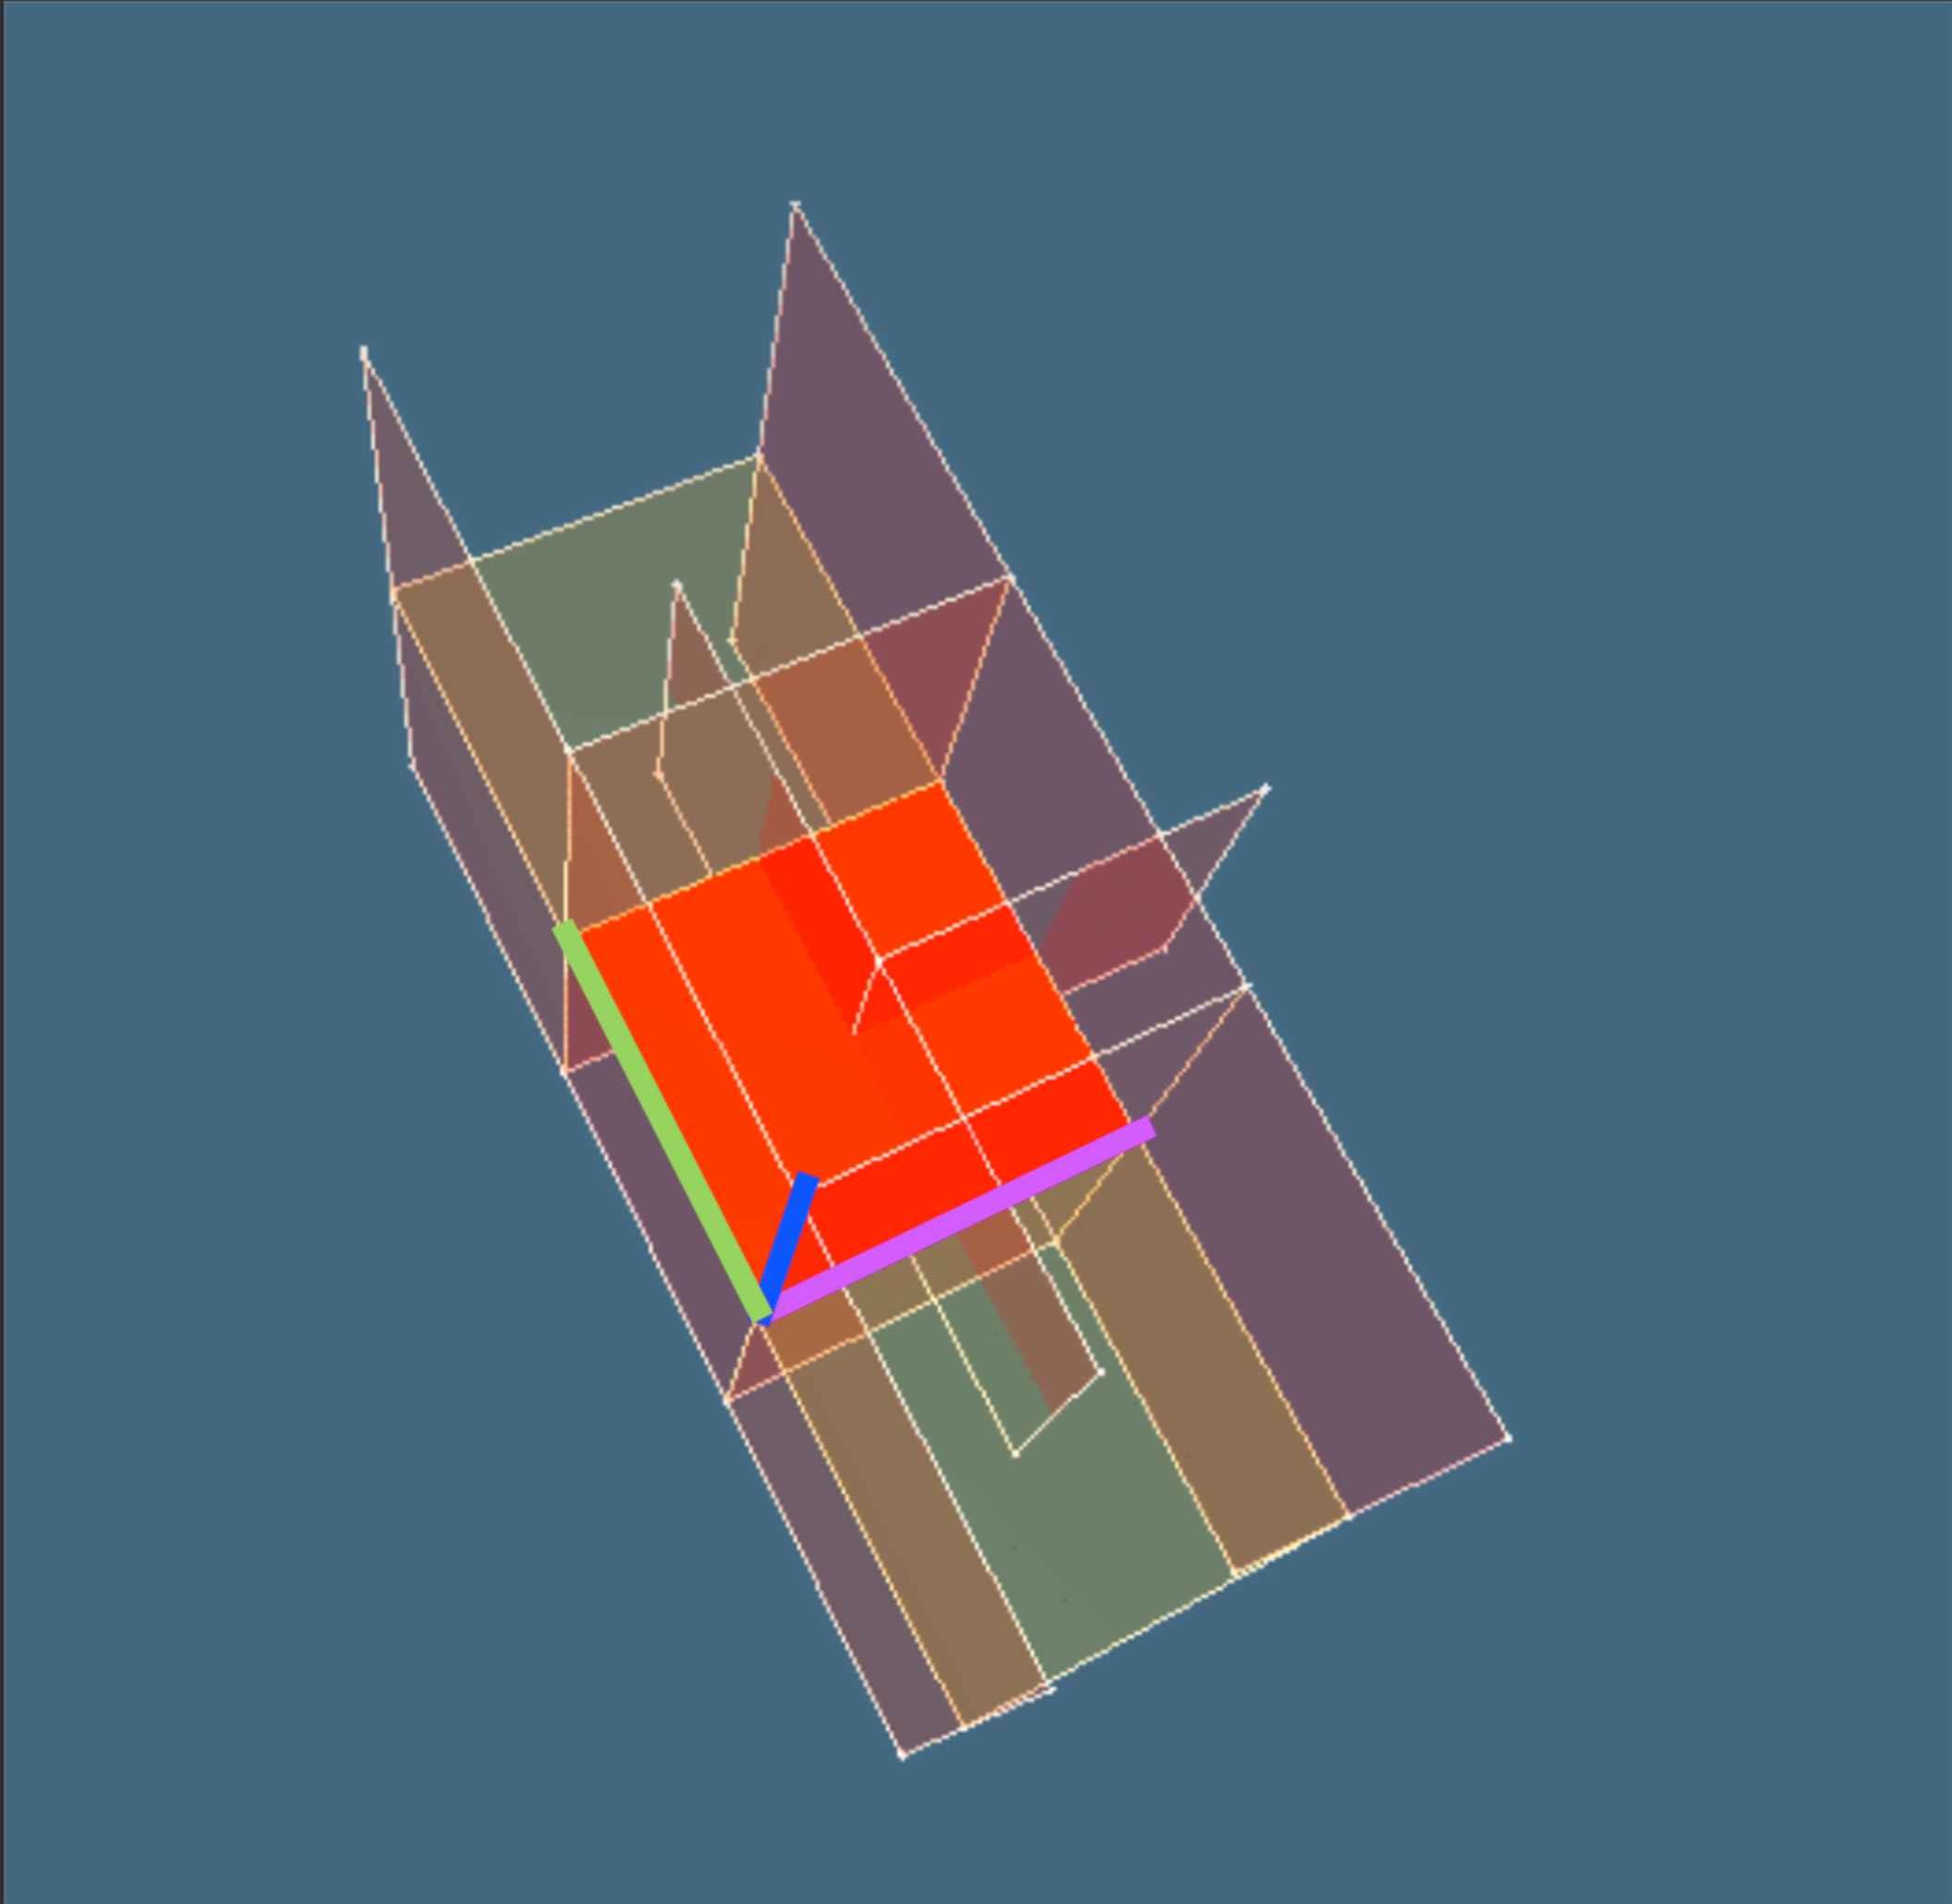
\includegraphics[width=0.49\textheight,width=0.47\textwidth]{submanifold3} 
   \caption{\emph{Submanifold mapping} of a 2-cell $f$ (red) and its  \texttt{bucket} \texttt{F[f]} of incident cells (transparent ones): (a) \texttt{F[f]} in \emph{world coordinates}; (b) \texttt{F[f]} in a local system, where $f$ is embedded in $z=0$ subspace.}
   \label{fig:testWall}
\end{figure}


\end{document}  